
\chapter{Solution Design }


\section{Introduction}

Reviewing the image-based approaches for wheat disease identification helped highlight the various techniques and models used to tackle the challenge of accurate disease recognition. This review provided valuable insights into the strengths and limitations of existing methods, guiding the development of a more tailored and effective solution. Building upon this analysis, we designed our solution to not only performs disease classification but also integrates complementary modules to address broader agricultural needs.

This chapter outlines the design of the proposed solution. It begins with a description of the overall system architecture, followed by details on dataset preparation and the deep learning models utilized for disease classification. In addition to the core classification component, the system incorporates two auxiliary modules: one for insect pest detection and another that provides users with assistance through a general-purpose AI assistant integrated via an external API.


\section{General design of the proposed solution}
Accurate detection of wheat diseases is essential for smart agriculture. While deep learning models show promise, many struggle with accurately predicting multiple disease classes. A major issue is the high false alarm rate, which incorrectly identifies healthy crops as diseased, leading to misdiagnosis, unnecessary interventions, and reduced trust in the system's reliability. Additionally, the similarity of symptoms across different fungal diseases often results in misclassification between disease types, which can cause farmers to choose inappropriate treatment methods, potentially worsening the situation or wasting resources.

The main goal of this work is to develop a robust deep learning solution capable of:
\begin{itemize}
    \item Detecting multiple wheat disease classes with high accuracy and recall, ensuring minimal false negatives (missed detections) and false positives (false alarms).
    \item Improving solution generalization across different environmental conditions (variations in lighting, backgrounds, and leaf positioning), image sources (e.g., drone, phone), and wheat varieties.
    \item Building an efficient solution suitable for integration into a  web platform for farmers.
\end{itemize}

To address the challenges identified during the literature review, our proposed classification solution leverages deep convolutional neural networks trained on high-resolution RGB images of wheat crops. The classification module is designed to accurately detect and distinguish between multiple wheat disease classes, even when symptoms appear visually similar. By carefully curating and augmenting the training dataset, we aim to improve model robustness against variations in lighting, image quality, background noise, and different wheat varieties. The system processes input images from diverse sources such as drones, cameras, or mobile phones, and outputs a reliable disease class prediction. This core classification module serves as the foundation of our approach, ensuring precision and scalability for real-world deployment.

To enrich the proposed solution and move toward a more holistic crop health monitoring system, additional modules were integrated into the system. One of these focuses on insect pest detection, as certain pests can be the primary cause of specific wheat diseases. Their early identification is crucial for addressing the root causes of infection and ensuring that treatment strategies target both symptoms and sources. Additionally, a general-purpose AI assistant was integrated via an API to support users by answering questions, guiding interpretation of results, and offering practical recommendations. Together with our proposed classification solution, these modules enhance the system’s ability to provide more accurate, timely, and context-aware support to farmers.

Figure 4.1 illustrates the global design of the proposed solution, including the main classification module and the two complementary modules. This figure also highlights the inputs and outputs of each module. It is important to note that the modules are separated and operate independently. The interaction between the AI assistant and the other two modules (wheat disease classification and pest detection) is entirely optional, giving users the freedom to engage with the assistant based on their specific needs or preferences.


\begin{figure}[H] % Requires \usepackage{float}
    \centering
    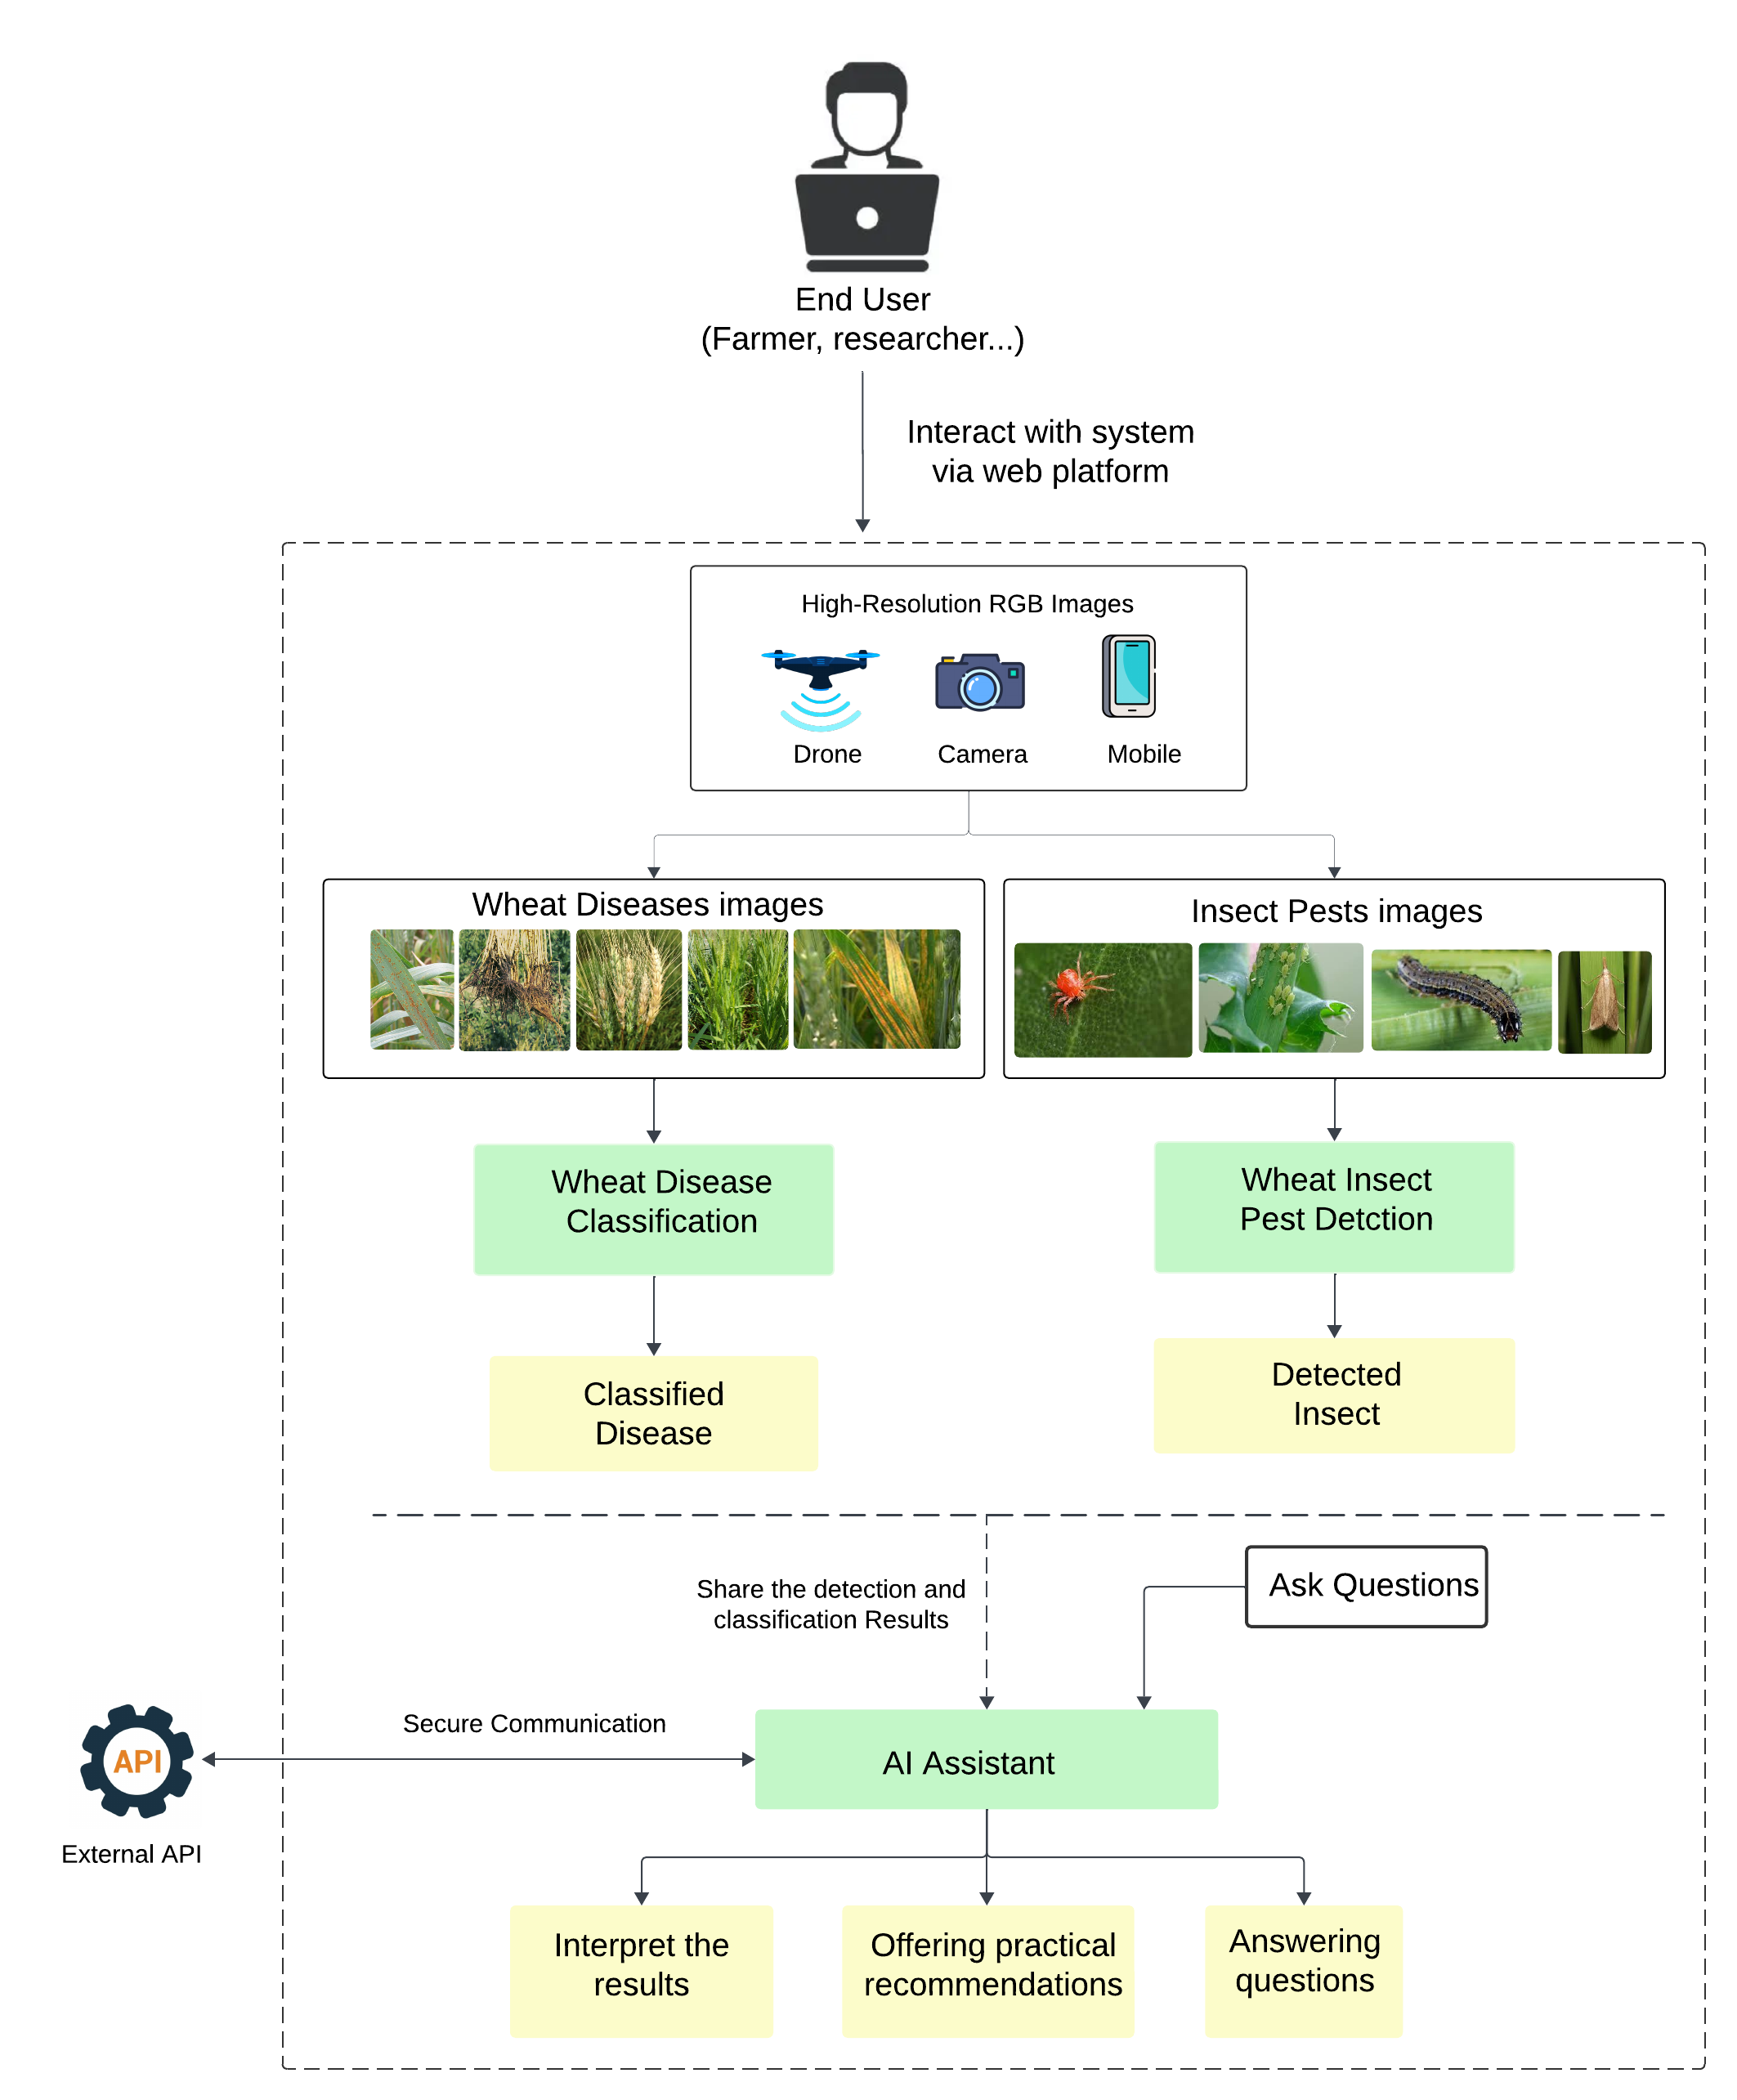
\includegraphics[width=\textwidth, height=0.99
    \textheight, keepaspectratio]{chapters/chapter4/images/Figure00.png}
    \caption{Block Diagram of the Proposed Multi-Module Wheat Monitoring System.}
    \label{fig:GlobalSys}
\end{figure}





\section{Detailed design of the proposed solution: Wheat disease classification}
This section outlines the methodology adopted for classifying wheat diseases, detailing the system's objectives, overall architecture, dataset design, and the models used in various classification scenarios.

\subsection{Global architecture overview}
The proposed solution adopts a two-stage classification pipeline. Once the input image is preprocessed, it is first passed through a binary classification model to determine the presence of disease. If the wheat plant is identified as diseased, a second model performs detailed diagnosis to identify the specific condition (See Figure ~\ref{fig:HierarchicalSystem}). The structure is described as follows:
\begin{itemize} 
    \item \textbf{Model 1 – Binary Classification:} This initial model determines whether the wheat plant is healthy or diseased. If the plant is classified as healthy, the system outputs a "Healthy" result and halts further processing.

    \item \textbf{Model 2 – Multiclass Classification:} If a disease is detected, this model takes over to identify the exact type of disease. It can classify the image into one of eight common wheat diseases: Yellow Rust, Brown Rust, Stem Rust, \Powdery Mildew, Loose Smut, Septoria, Fusarium,  Tan Spot and Common Root Rot.
\end{itemize}

\begin{figure}[H] % 'H' needs \usepackage{float}
    \centering
    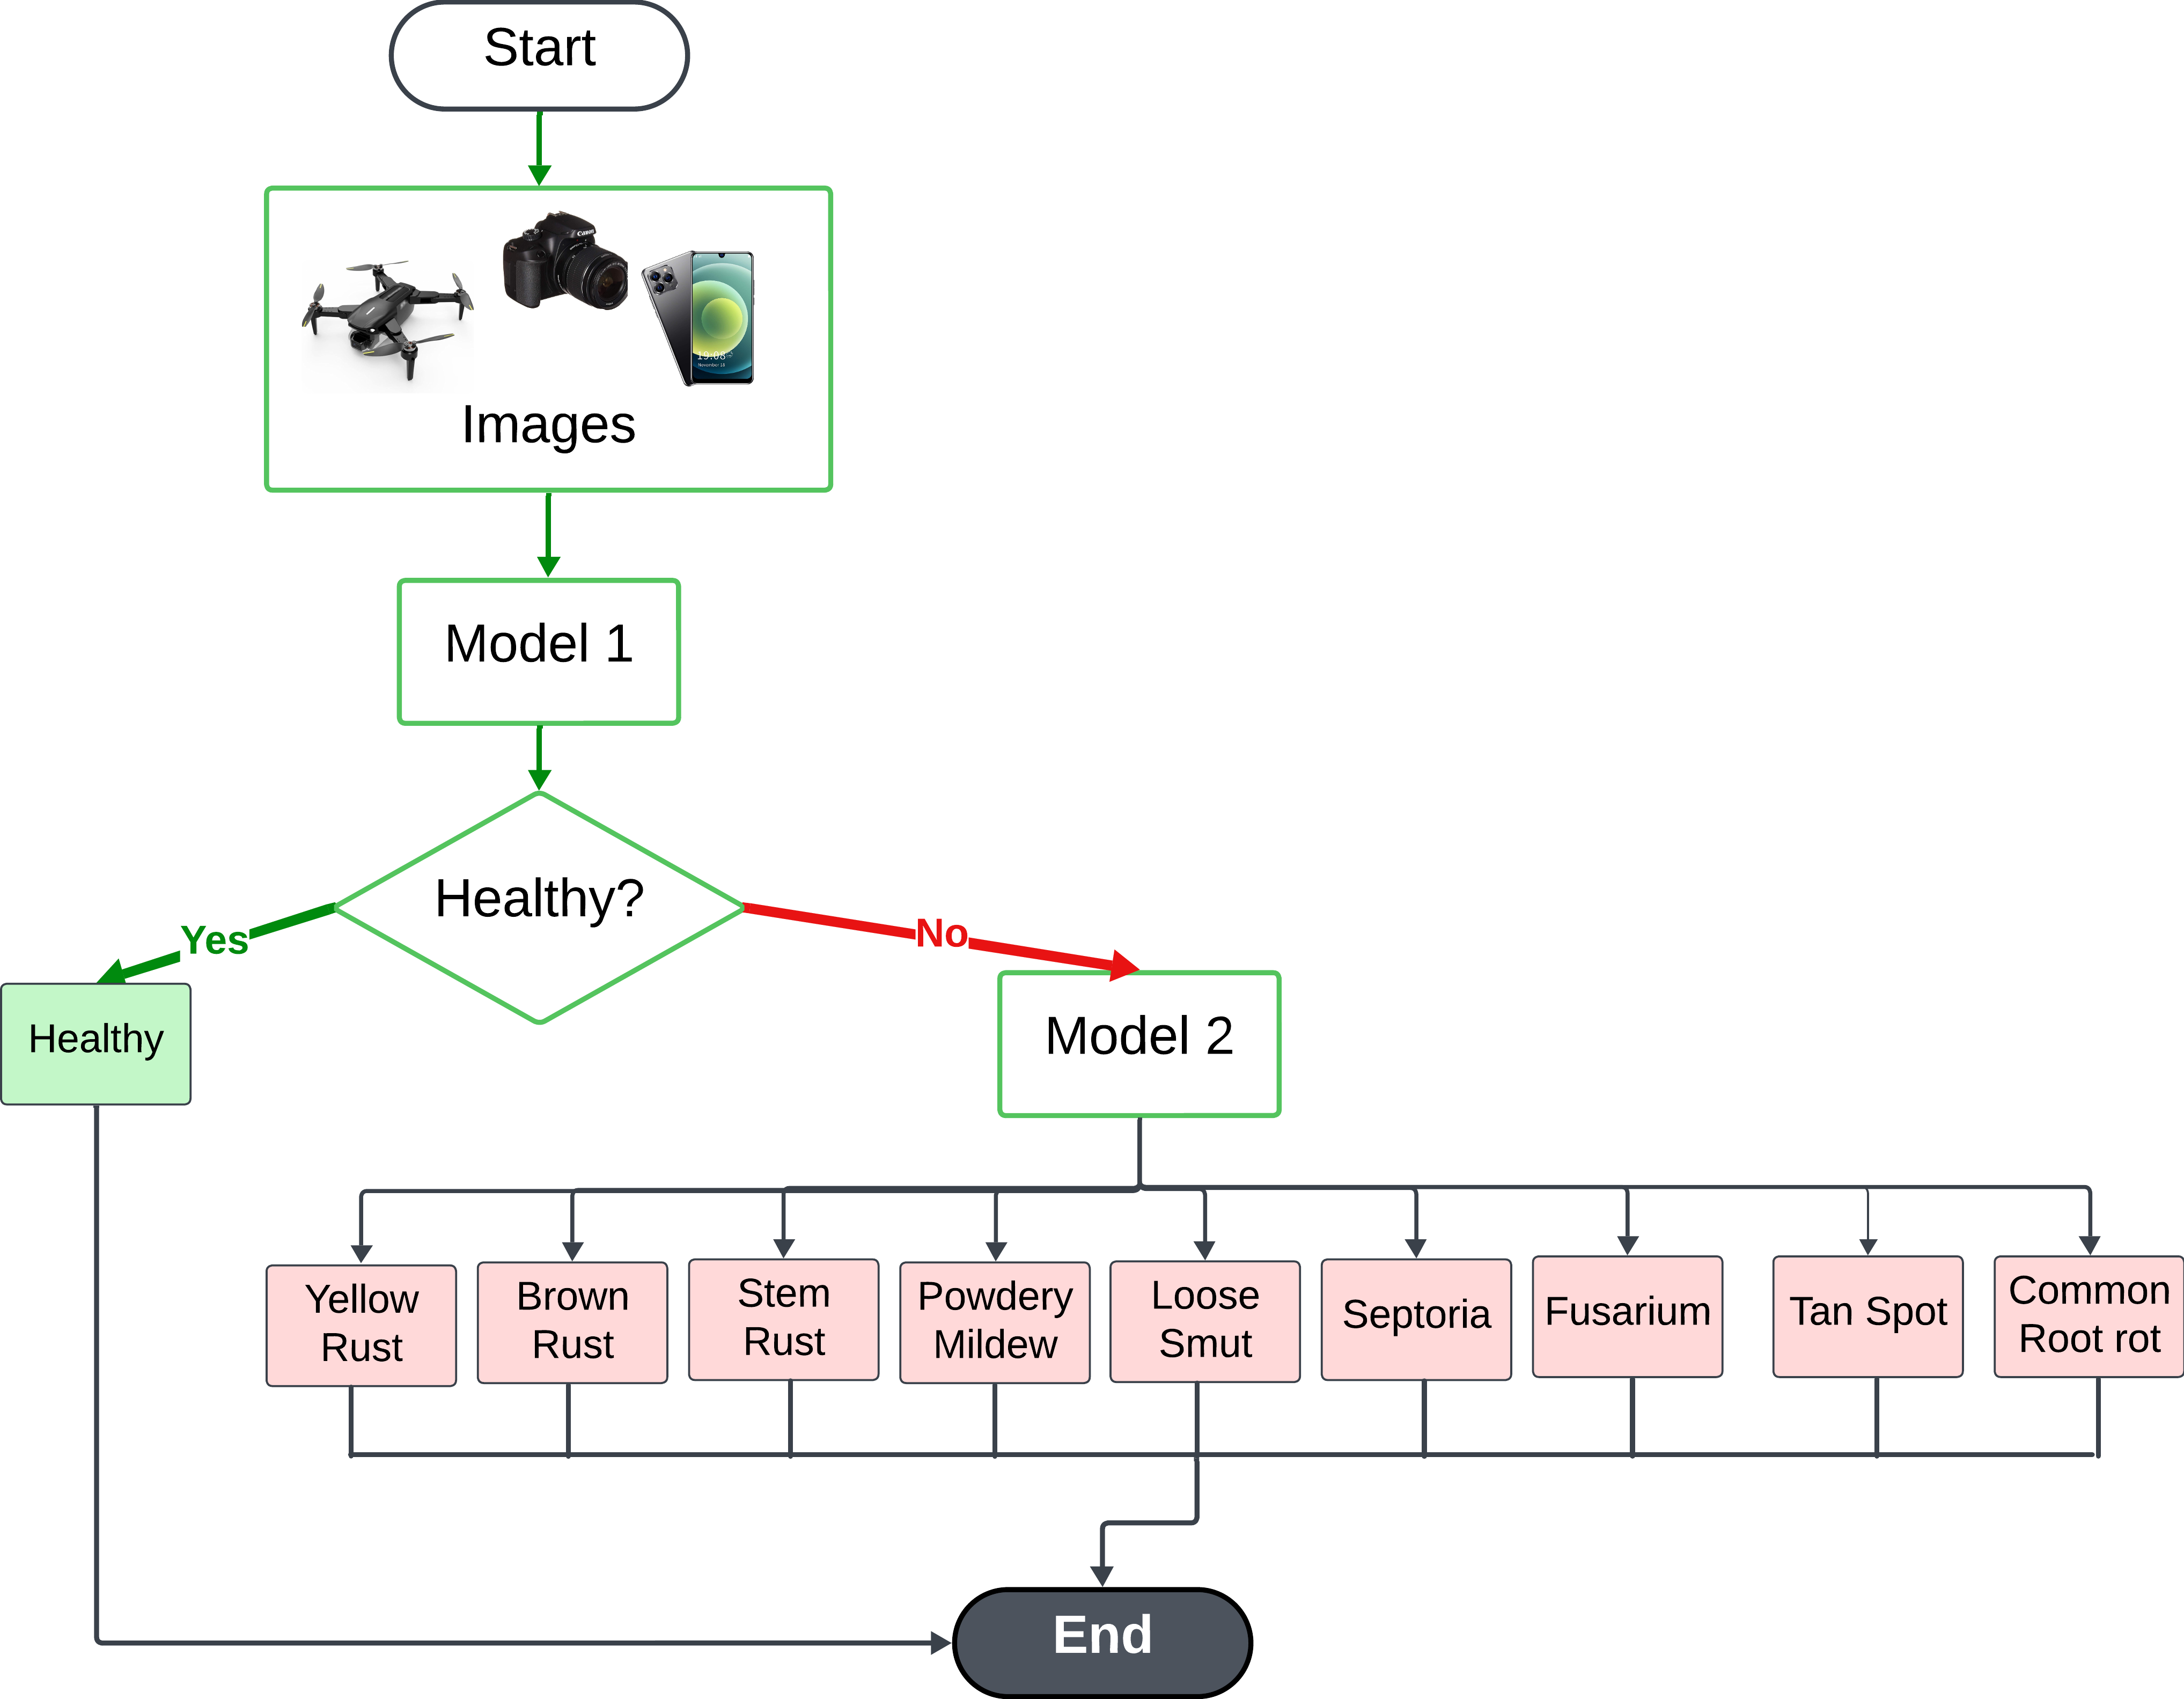
\includegraphics[width=0.8\textwidth]{chapters/chapter4/images/Figure01.png}
    \caption{Hierarchical system for wheat disease classification.}
    \label{fig:HierarchicalSystem}
\end{figure}

Now it is  to explain the reason behind adopting a hierarchical classification approach instead of relying on a single multiclass model to detect and classify wheat diseases directly. We arrived at this approach after conducting several initial experiments using a single-stage multiclass model. Although it provided promising results, we observed certain limitations, especially in cases where healthy plants were misclassified as diseased (Results are presented in Section~\ref{sec:justifyHAmodel})
when rare disease classes were not detected accurately due to class imbalance.

This led us to explore a hierarchical strategy, which divides the task into two more focused stages: first identifying whether a plant is diseased or not, and then determining the specific disease. This structure offers several advantages:

\begin{itemize}
\item \textbf{Improved accuracy:} By separating the detection of disease from the identification of its type, each model becomes more specialized and performs better on its specific task.

\item \textbf{Interpretability and efficiency:} If the plant is classified as healthy by the binary classifier, the system halts further processing. This avoids unnecessary computations and helps reduce the risk of false positives in the second stage.

\item \textbf{Better handling of class imbalance:} In agricultural datasets, healthy samples often dominate. The binary model filters out these cases, allowing the second model to focus only on distinguishing between disease types.

\item \textbf{Reducing computational complexity:} Only diseased samples undergo detailed classification, which minimizes unnecessary computation.
\end{itemize}

\subsection{Wheat disease dataset construction}
Various public datasets for wheat disease detection are available online through platforms like Kaggle, GitHub, and Google Drive. These datasets typically contain images representing a few disease classes, but the image counts and quality vary significantly. Common issues include low-resolution or blurred images, misclassified or irrelevant samples, redundant (duplicate) images, and limited class diversity often covering only two to four disease types. Additionally, some datasets contain images that are not only unrelated to the disease but also have no clear connection to wheat itself, which can introduce noise and reduce model performance. Moreover, most images are captured at close range, which limits the model’s ability to generalize to field-level scenarios,  such as those involving RGB drone imagery.
\begin{table}[htbp]
    \caption{Overview of used wheat disease datasets}
    \centering
    \resizebox{\textwidth}{!}{%
    \begin{tabular}{|p{4cm}|p{2cm}|p{6cm}|p{3.5cm}|}
    \hline
    \textbf{Dataset} & \textbf{Source} & \textbf{Classes} & \textbf{Size} \\
    \hline
    Wheat Leaf Dataset & Mendeley Data & Healthy (102), Stripe Rust (208), Septoria (97) & 407 images \\
    \hline
    Wheat Disease Detection & Kaggle & Healthy (1116), Yellow Rust (924), Brown Rust (902) & 2942 images \\
    \hline
    Wheat Fungi Diseases Dataset (WFD 2020) & \parencite{genaev2021} &Healthy (517), Yellow Rust (457), Stem Rust(388),  Septoria (185), Leaf Rust (655), Powdery Mildew (277), seedling (255) & 2734 images \\
    \hline
    CGIAR & Kaggle & Healthy (142), Leaf Rust (358), Stem Rust (376) & 876 images \\
    \hline
    LWDCD 2020 & Google Drive & Crown and Root Rot (1040), Fusarium Head Blight (1270), Healthy (1280), Leaf Rust (1620) & 5210 images \\
    \hline
    Wheat Disease Dataset WDD 2017 & Kaggle & Brown Rust (166), Healthy (242), Loose Smut (99), Septoria (34), Yellow Rust (195) & 736 images \\
    \hline
    \end{tabular}%
    }
    \label{tab:wheat-datasets}
\end{table}

To overcome the limitations of existing datasets, we constructed a custom wheat disease dataset by carefully curating and filtering images from multiple publicly available sources (Table~\ref{tab:wheat-datasets}). This involved eliminating low-quality or irrelevant samples, correcting mislabeled entries, and ensuring visual diversity, particularly in terms of image acquisition angles and capture distances (e.g., close-up and aerial views). The primary objective was to build a robust and representative dataset capable of supporting accurate and generalizable classification under diverse real-world conditions. Our final dataset comprises 3863 images spanning ten distinct classes: Healthy, Yellow Rust, Stem Rust, Brown Rust, Powdery Mildew, Septoria, Loose Smut, Fusarium, Tan Spot and Common Root Rot (Figure~\ref{fig:ourcustomdataset}).

\begin{figure}[H] % 'H' needs \usepackage{float}
    \centering
    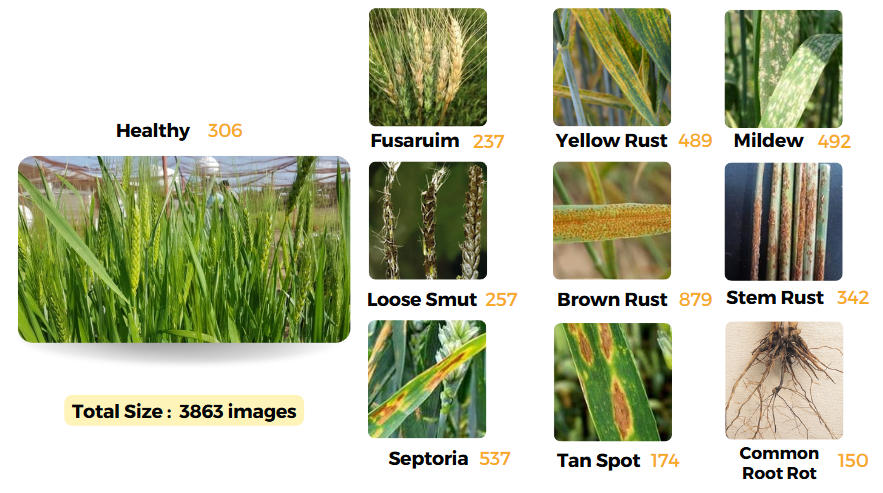
\includegraphics[width=0.9\textwidth]{chapters/chapter4/images/Figure02.png}
    \caption{Sample images from our custom dataset.}
    \label{fig:ourcustomdataset}
\end{figure}

To support the development and training of the hierarchical classification system, the dataset was strategically divided into two subsets: D1 and D2, designated for Model 1 (the binary classifier) and Model 2 (the multi-class classifier), respectively. For D1, a balanced distribution was ensured by randomly selecting 410 images labeled as Not Healthy drawn from the nine disease categories and pairing them with 306 images labeled as Healthy. This balance was essential for effective binary classification. In contrast, D2 was constructed to include only the disease classes, explicitly excluding the Healthy category.

\subsection{Binary classification model}


Before defining the architecture of the binary classification model, it is important to note that its construction went through several experimental phases. Multiple tests and evaluations were conducted to explore different configurations, allowing us to determine the most effective architecture in terms of performance and efficiency. Various model configurations, preprocessing strategies, and feature extraction methods were evaluated in order to strike a balance between accuracy, generalization, and computational efficiency.
The final adopted pipeline consists of three main steps: data preparation. feature extraction and finally the classification. The architecture of this model with all its steps is presented in Figure~\ref{fig:binaryClassification}.To understand this proposed architecture, let's break down its main steps: 

\begin{figure}[H] % 'H' needs \usepackage{float}
    \centering
    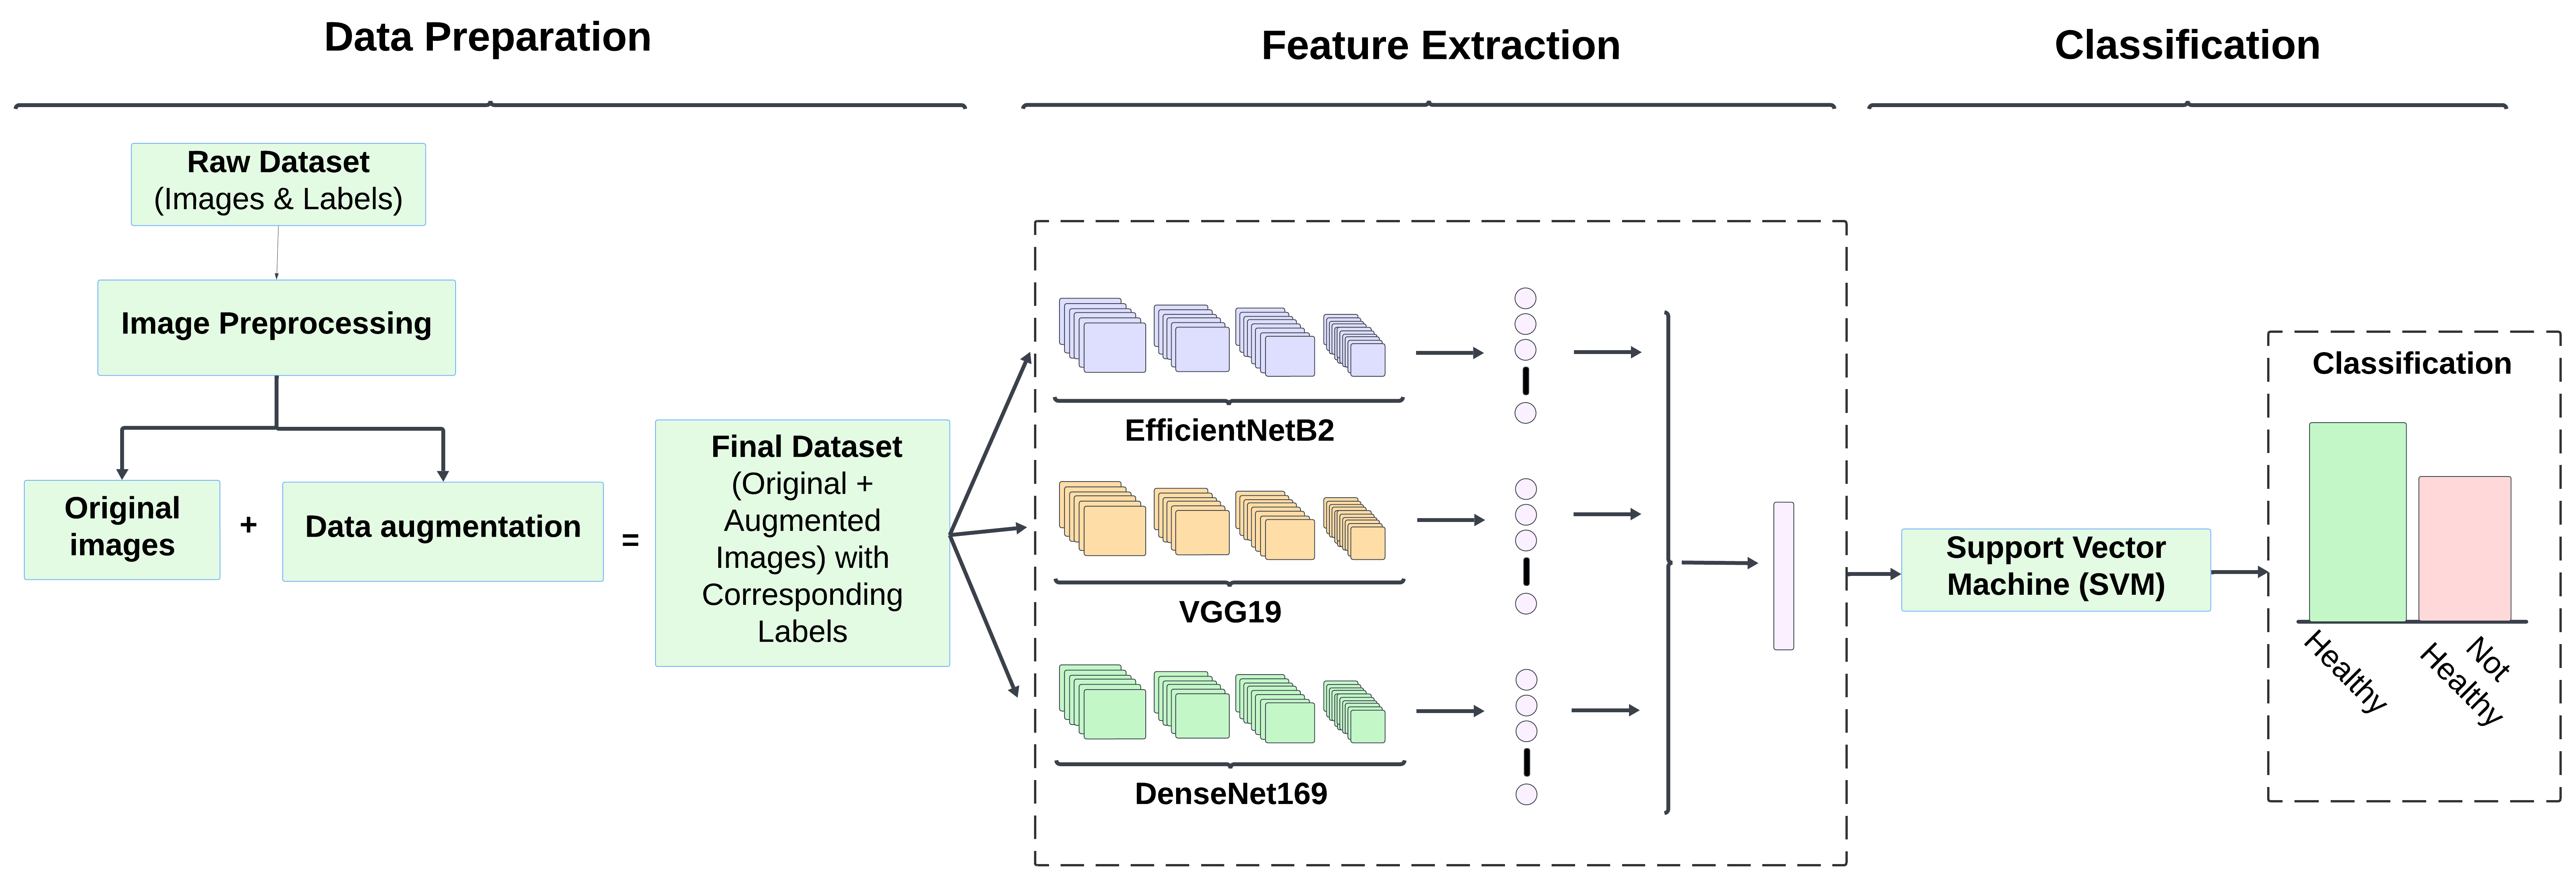
\includegraphics[width=1.1\textwidth]{chapters/chapter4/images/Figure03.png}
    \caption{Architecture of the binary classification model.}
    \label{fig:binaryClassification}
\end{figure}

\subsubsection{Data preparation:} 
The preparation of data is a fundamental step in building an effective classification system. In this phase raw dataset undergoes preprocessing to standardize image quality and ensure uniformity across all samples. Each image is resized to 224×224 pixels, a common input size required by several modern deep learning architectures. This resizing also ensures compatibility with the pre-trained models selected for feature extraction in our model.
The dataset is then divided into training and testing sets, with 80\% allocated for training and 20\% for testing. To further enhance the model’s generalization ability and reduce the risk of overfitting, we apply a set of well-established data augmentation techniques. These techniques are defined in Table~\ref{tab:DataAugmentation}. They include:
\begin{table}[h]
    \caption{Data augmentation techniques and parameters.}
    \centering
    \renewcommand{\arraystretch}{1.5}
    \setlength{\tabcolsep}{10pt}
    \begin{tabular}{|p{3.5cm}|p{6.5cm}|p{4cm}|}
        \hline
        \textbf{Technique} & \textbf{Description} & \textbf{Parameter Configuration} \\ \hline
        Gamma Correction & Adjusts image brightness non-linearly to simulate lighting variations & Gamma ($\gamma$) = 1.5 \\ \hline
        CutOut & Randomly masks square regions of the image to prevent overfitting & Mask size = 50×50 px \\ \hline
        MixUp & Blends two images and labels to improve generalization & Alpha ($\alpha$) = 0.2 \\ \hline
        CutMix & Cuts and pastes a patch from one image into another to simulate occlusion & Alpha ($\alpha$) = 1.0 \\ \hline
    \end{tabular}-
    \label{tab:DataAugmentation}
\end{table}
Each technique is applied with carefully chosen parameters, contributing to increased variability in the training data. As illustrated in Figure~\ref{fig:DataaugmentationExemple}, these transformations generate realistic variations of the original images. The final training set combines both the original and augmented images, all paired with their corresponding labels, forming a richer and more diverse dataset.


\begin{figure}[H] % 'H' needs \usepackage{float}
    \centering
    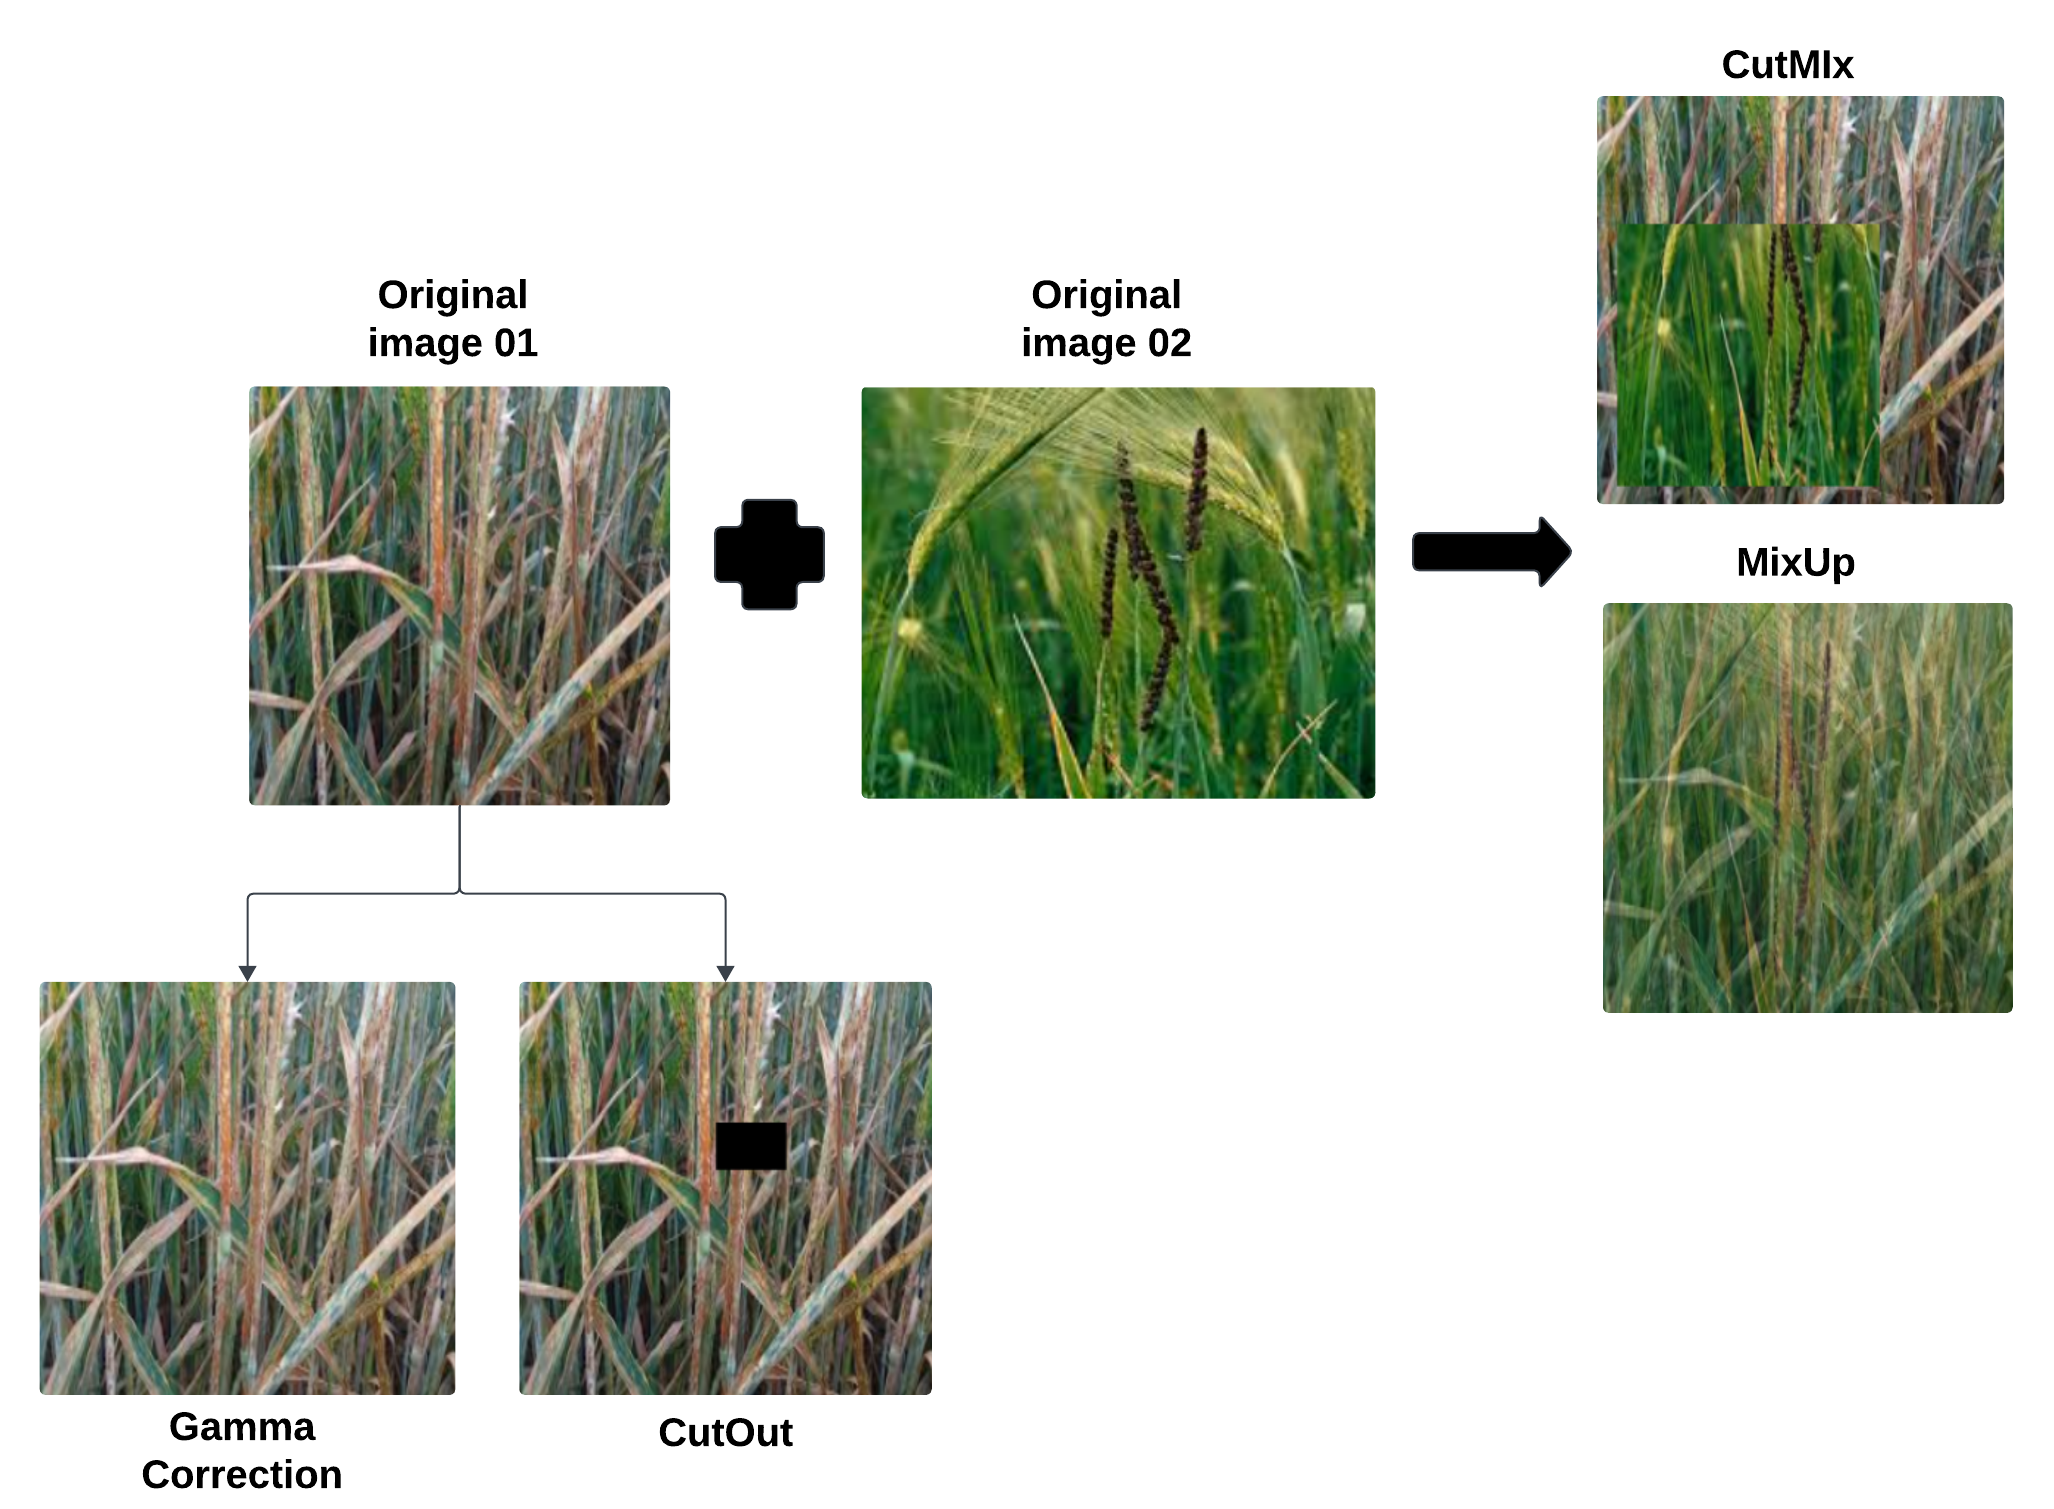
\includegraphics[width=0.8\textwidth]{chapters/chapter5/images/Figure01.png}
    \caption{Data augmentation techniques (Example of application).}
    \label{fig:DataaugmentationExemple}
\end{figure}

In addition, Figure~\ref{fig:Model2Dataaugmentation} shows the class distribution after augmentation. A balanced number of samples for each class is maintained, particularly between the \textit{Healthy} and \textit{Not Healthy} categories, which is critical for avoiding bias during training and ensuring that the model learns to distinguish between classes effectively.
\begin{figure}[H] % 'H' needs \usepackage{float}
    \centering
    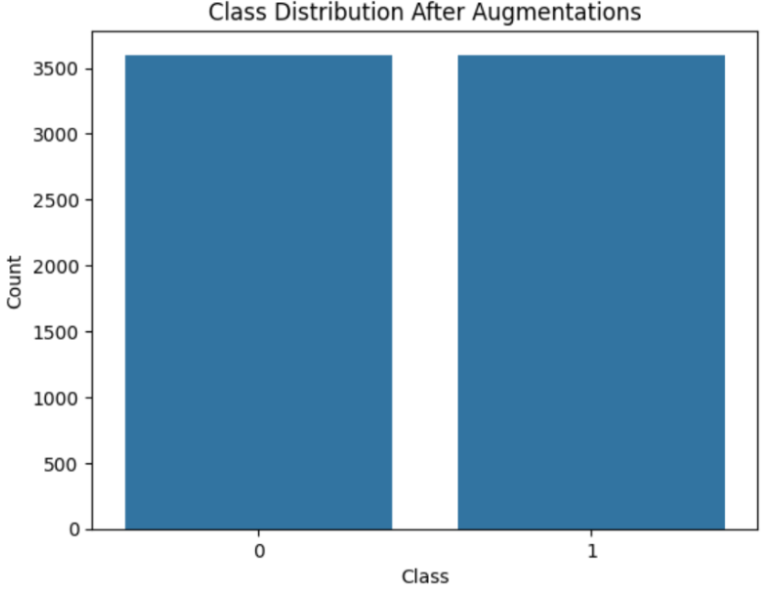
\includegraphics[width=0.8\textwidth]{chapters/chapter5/images/Figure02b.png}
    \caption{Class Distribution After Augmentation..}
    \label{fig:Model2Dataaugmentation}
\end{figure}

\vspace{0.3cm}
\subsubsection{Feature Extraction:} 
To effectively capture meaningful patterns from the dataset and improve classification performance, we leveraged state-of-the-art pre-trained convolutional neural networks (CNNs) for feature extraction. Using pre-trained models offers two key advantages: it reduces computational cost by reusing learned filters from large-scale datasets, and it help to enhance the performance as these models have already learned to recognize generic visual features like edges, textures, and shapes.

This approach is particularly important for our binary classification task, where the Not Healthy class includes a wide range of distinct wheat diseases. Each disease manifests with different visual symptoms such as spots, discolorations, or irregular patterns which require the extraction of diverse and discriminative features to ensure accurate classification. A single pretrained model might not capture all these variations effectively, which motivated the use of multiple feature extractors.

The selection of the final set of feature extractors was guided by empirical evaluation. Several pre-trained CNN architectures were tested and compared on the dataset D1. As a result of this evaluation process, three models were selected: EfficientNetB2, VGG19, and DenseNet169. These models demonstrated strong and consistent performance (Tests results are presented in this section~\ref{sec:testcnnModel1}).

To implement the feature extraction process, several key configurations were adopted:
\begin{itemize}
    \item A batch size of 32 is used throughout the extraction process to balance computational efficiency and memory usage.


    \item Feature extraction is carried out using the selected models, all pre-trained on \textit{ImageNet}, which provides a robust initialization and supports faster convergence.

    \item Model adaptation is performed by setting the \texttt{include\_top} parameter to \texttt{false}, removing the original classification head of each model. This allows the networks to be repurposed solely for feature extraction in our classification context.

    \item After feature extraction, a \texttt{GlobalAveragePooling2D} layer is applied. This layer reduces the spatial dimensions by averaging each feature map, resulting in a compact 1D feature vector that preserves the most significant information while reducing the risk of overfitting.

\end{itemize}
\vspace{0.3cm}
\subsubsection{Classification:} 
After feature extraction, the concatenated feature vectors are fed into a traditional machine learning classifier to perform the binary classification task. At this stage, the classification involves only two classes: Healthy and Not Healthy.

So instead of relying on deep learning-based end-to-end classifiers, we opted to use traditional machine learning (ML) algorithms for several reasons:
\begin{itemize}
    \item The task at this stage is a \textbf{binary classification problem}, which simplifies the decision boundary and aligns well with the strengths of classical ML methods.
    
    \item ML algorithms are generally \textbf{faster to train} and \textbf{less computationally intensive} compared to deep learning models.
    
    \item They are particularly \textbf{effective when used with high-quality, pre-extracted features}, such as those obtained from pre-trained CNNs.
\end{itemize}

To identify the most suitable classifier, we conducted  also here empirical tests using the dataset D1. The models evaluated include: \gls{abb:mlp}, \gls{abb:dt}, \gls{abb:rf} and \gls{abb:svm}. Performance was assessed using standard evaluation metrics such as accuracy and F1-score (see the next chapter for detailed results in this section~\ref{sec:MLclassifiertest}). Among these, the Support Vector Machine (SVM) yielded the best performance and was therefore selected as the final classifier. 

Support Vector Machine (SVM) is a powerful supervised machine learning algorithm widely used for classification and regression tasks due to its efficiency and ability to manage high-dimensional data. At its core, SVM aims to find the optimal hyperplane that best separates data points from two classes by maximizing the margin, the distance between the hyperplane and the nearest data points, known as support vectors. When data is not linearly separable, SVM applies the "kernel trick" to map inputs into a higher-dimensional space where a linear separation becomes feasible (Figure~\ref{fig:SVM}); common kernel functions include linear, polynomial, radial basis function (RBF), and sigmoid \parencite{guido2024}.

\begin{figure}[H] % 'H' needs \usepackage{float}
    \centering
    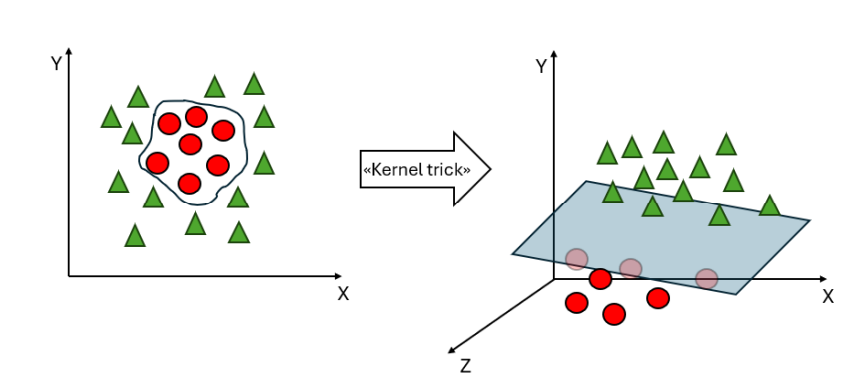
\includegraphics[width=0.9\textwidth]{chapters/chapter4/images/Figure04.png}
    \caption{An example of the “kernel trick” \parencite{guido2024}.}
    \label{fig:SVM}
\end{figure} 


Then a systematic hyperparameter optimization was conducted using \texttt{GridSearchCV}. This approach combines exhaustive grid search, which evaluates all possible combinations of specified hyperparameters, with cross-validation to ensure reliable and unbiased performance estimation. Specifically, 3-fold cross-validation was employed, where the training data is partitioned into three subsets; in each iteration, two subsets are used for training while the remaining one is used for validation. This process is repeated three times, and the performance metrics are averaged to reduce overfitting and ensure the model generalizes well to unseen data.

To improve computational efficiency, parallel processing was enabled by setting n\_jobs set to -1, allowing the use of all available CPU cores during the grid search process. Additionally, for scenarios involving class imbalance, the \texttt{class\_weight} parameter was set to \texttt{"balanced"}, automatically adjusting weights inversely proportional to class frequencies in the training set.

Key hyperparameters for the SVM classifier were tuned to identify the optimal configuration, as summarized in Table~\ref{tab:svm_grid}. These include the regularization parameter \texttt{C}, kernel type, kernel coefficient \texttt{gamma}, and polynomial \texttt{degree} (relevant when using a polynomial kernel). These parameters were selected based on their significant impact on the SVM’s decision boundary and generalization ability.

\begin{table}[h]
\centering
\caption{Grid search configuration of SVM classifier hyperparameters}
\begin{tabular}{|p{4.5cm}|p{8.5cm}|}
\hline
\textbf{Hyperparameters} & \textbf{Explored Values} \\
\hline
C (Regularization parameter) & \{0.1, 1, 10\} \\
\hline
Kernel (type of kernel function) & \{linear, rbf, poly\} \\
\hline
gamma (kernel coefficient) & \{scale, auto\} \\
\hline
degree (polynomial degree) & \{2, 3, 4\} \\
\hline
\end{tabular}
\label{tab:svm_grid}
\end{table}

After conducting the grid search with cross-validation, the best-performing configuration for the SVM classifier was identified, as shown in Table~\ref{tab:svm_best}. These hyperparameters were selected based on their cross-validated performance and were used in the final ensemble to ensure optimal and consistent results.

\begin{table}[h]
\centering
\caption{Best hyperparameter settings selected by Grid Search for SVM classifier}
\begin{tabular}{|p{4.5cm}|p{8.5cm}|}
\hline
\textbf{Hyperparameters} & \textbf{Selected Values} \\
\hline
C & 10 \\
\hline
kernel & rbf \\
\hline
gamma & scale \\
\hline
degree & 2 \\
\hline
\end{tabular}
\label{tab:svm_best}
\end{table}

After explaining all the components of the binary classification model M1, we now present the algorithm summarizing the overall process used for training and inference.




\begin{algorithm}[H]
\caption{Binary Classification Model (M1)}
\textbf{Input:} Image dataset $\mathcal{D} = \{(x_i, y_i)\}_{i=1}^{N}$, where $N$ is the total number of image samples, $x_i$ represents the $i$-th image of a wheat plant, and $y_i$ is the corresponding binary label. The label $y_i \in \{0, 1\}$ indicates the health status of the plant: $y_i = 0$ denotes a healthy wheat plant, and $y_i = 1$ denotes a diseased (unhealthy) wheat plant\;
\textbf{Output:} Trained SVM classifier $f(x)$\;

\vspace{2mm}
\textbf{Step 1: Data Preparation}\;
\ForEach{image $x_i \in \mathcal{D}$}{
    Resize $x_i$ to $224 \times 224$\;
    Normalize pixel values\;
}
Apply data augmentation techniques:\;
\Indp
Gamma Correction\;
CutOut\;
MixUp\;
CutMix\;
\Indm
Construct augmented dataset $\mathcal{D}_{\text{aug}}$ by combining original and augmented samples\;
Split $\mathcal{D}_{\text{aug}}$ into $D_{\text{train}}$ (80\%) and $D_{\text{test}}$ (20\%)\;

\vspace{2mm}
\textbf{Step 2: Feature Extraction}\;
\ForEach{image $x_i \in D_{\text{train}}$}{
    \ForEach{CNN model $M \in \{$EfficientNetB2, VGG19, DenseNet169$\}$}{
        Load $M$ with ImageNet weights and remove the final ImageNet classification layers\;
        Apply GlobalAveragePooling to extract feature vector $f^M_i$\;
    }
    Concatenate features: $f_i = [f_i^{\text{EffNet}} \| f_i^{\text{VGG}} \| f_i^{\text{DenseNet}}]$\;
}
Build feature matrix $F_{\text{train}}$ and label vector $Y_{\text{train}}$\;

\vspace{2mm}
\textbf{Step 3: Classification}\;
Define Grid Search Configuration:\;
\Indp
Regularization parameter $C$, kernel type, kernel coefficient $\gamma$, and polynomial degree\;
\Indm
Use GridSearchCV with 3-fold cross-validation on $(F_{\text{train}}, Y_{\text{train}})$\;
Train final model $f(x)$ using best configuration\;
\vspace{1mm}
\textbf{Return:} Final trained SVM classifier $f(x)$\;
\end{algorithm}




















\subsection{Multi-class Classification Model}

Similar to the binary classification model, various empirical tests were conducted to determine the optimal architectural design for the multi-class classification model. The development of this model involved several key stages, including data preprocessing techniques, feature extraction and classification. The overall architecture and data flow of the model are illustrated in Figure~\ref{fig:Multiclassclassification}. Let's break down each component to gain a better understanding of this architecture:


\begin{figure}[H] % 'H' needs \usepackage{float}
    \centering
    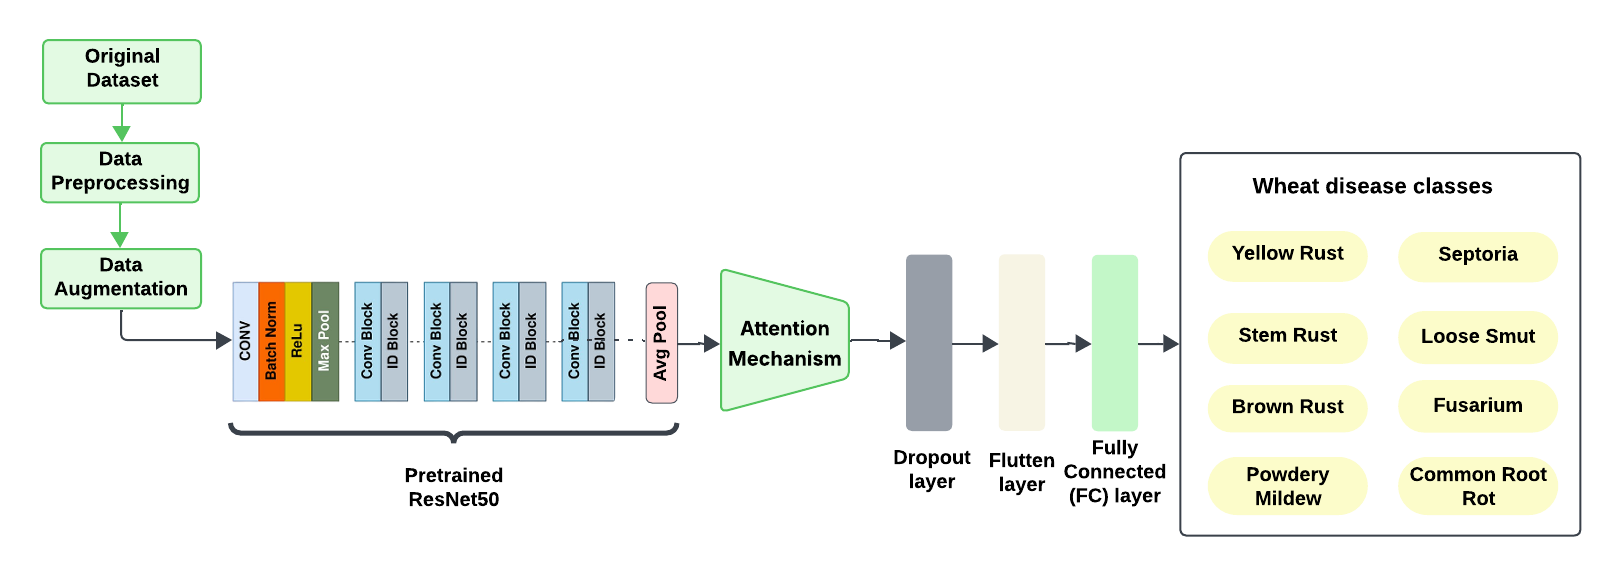
\includegraphics[width=1\textwidth]{chapters/chapter4/images/Figure05.png}
    \caption{Architecture of the multi-class wheat disease classification model.}
    \label{fig:Multiclassclassification}
\end{figure}



\subsubsection{Data preprocessing:} 
\label{sec:data_augmentation}
This stage begins with standard image preprocessing techniques, including resizing to a uniform input size, random cropping to introduce spatial variability, and normalization to scale pixel values. These operations ensure consistency across the dataset and reduce input variance, thereby enhancing the model’s generalization capability.

To facilitate effective training and unbiased evaluation, the dataset was divided into three subsets: 70\% for training, 15\% for validation, and 15\% for testing. This stratified split enables reliable performance monitoring and assessment on unseen data.

Comprehensive augmentation strategies were applied to further improve the robustness of the classification model, these augmentations are seamlessly integrated during the data loading phase. For the training set, the preprocessing pipeline includes geometric transformations (resizing, random cropping, rotation, flipping, and shifting), color adjustments (brightness, contrast, hue, saturation), and noise simulation (Gaussian blur), followed by normalization and conversion to tensors. In contrast, validation and test images undergo a simpler pipeline consisting only of resizing and normalization to preserve data fidelity.

The impact of these transformations is illustrated in Figure~\ref{fig:VisualExamples}, while the exact augmentation parameters are summarized in Table~\ref{tab:ImagePreprocessingConfig}, offering a clear overview of the configurations settings.


\begin{figure}[H] % 'H' needs \usepackage{float}
    \centering
    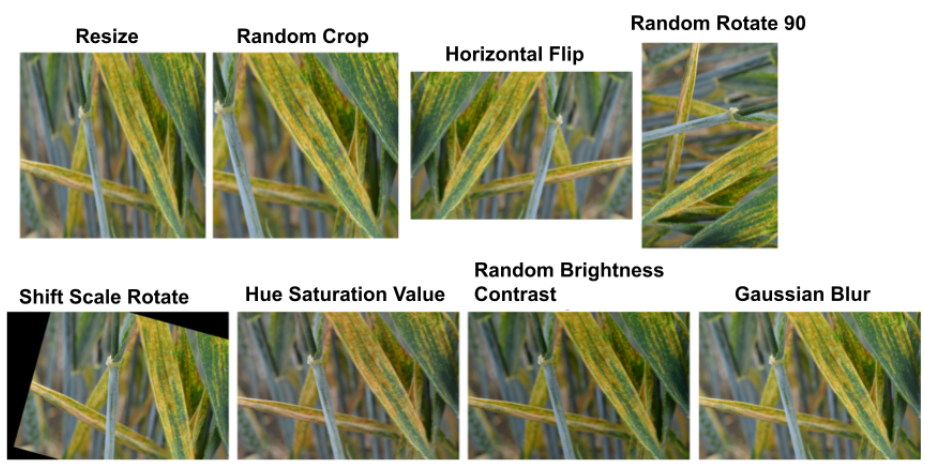
\includegraphics[width=0.9\textwidth]{chapters/chapter5/images/Figure08.png}
    \caption{Visual Examples of Image Variations Generated Through Data Augmentation Techniques.}
    \label{fig:VisualExamples}
\end{figure}


\begin{table}[ht]
\centering
\caption{Configuration of parameters for image preprocessing and augmentation techniques.}
\renewcommand{\arraystretch}{1.3}
\begin{tabular}{|l|p{9cm}|}
\hline
\textbf{Data Processing Technique} & \textbf{Parameter(s) and Value(s)} \\
\hline
Resize & Height: 512, Width: 512 \\
\hline
Random Crop & Height: 448, Width: 448 \\
\hline
Horizontal Flip & Probability: 0.5 \\
\hline
Random 90° Rotation & Probability: 0.5 \\
\hline
Shift, Scale, Rotate & Shift limit: 0.1, Scale limit: 0.1, Rotate limit: 20°, Probability: 0.5 \\
\hline
Hue, Saturation, Value Shift & Hue limit: ±10, Saturation limit: ±15, Value limit: ±10, Probability: 0.5 \\
\hline
Brightness and Contrast & Probability: 0.5 \\
\hline
Gaussian Blur & Blur limit: 3, Probability: 0.3 \\
\hline
Normalize & Mean: (0.485, 0.456, 0.406), Std: (0.229, 0.224, 0.225) \\
\hline
\end{tabular}
\label{tab:ImagePreprocessingConfig}
\end{table}




\subsubsection{Feature extraction:}  
This stage involves a more complex multi-class classification problem, where the dataset \textit{D2} includes a significantly larger number of images and encompasses nine distinct disease classes. To address this complexity and improve the model’s ability to generalize, we employed pre-trained convolutional neural networks. 

To select the most suitable architecture for this task, we tested several pre-trained CNN models (EfficientNetB2, MobileNet, Xception, InceptionV3, DenseNet201 and ResNet50V2) on the augmented dataset \textit{D2}. As detailed in this section~\ref{sec:TestCnnM2}, these empirical evaluations demonstrated that ResNet50V2 outperformed the others CNN models. Therefore, it was selected as the backbone feature extractor in this model, and it operates as follows:
\begin{itemize}
    \item Input images are processed through multiple convolutional blocks (Conv Blocks), followed by identity blocks (ID Blocks), ReLU activations, batch normalization, and max pooling layers to extract deep hierarchical features.
    \item Pre-trained weights from ImageNet enable the model to efficiently capture complex visual patterns associated with different wheat diseases.
    \item A Global Average Pooling layer is applied at the end to reduce the dimensionality while preserving the most informative features for classification.
\end{itemize}

However, the visual similarity between certain disease classes such as yellow rust and brown rust, or Septoria and Tan Spot makes it particularly challenging for the model to accurately distinguish between them. So relying on global feature representations may not be sufficient. Subtle differences in symptom patterns can easily be overlooked if all channels are treated equally. To further refine the extracted features and emphasize discriminative patterns, we integrate an attention mechanism along with the preterined model. This mechanism helps to focus on the most relevant features and suppress less informative signals.


We incorporated the Efficient Channel Attention (ECA) module after empirical evaluations demonstrated its superior performance compared to other attention mechanisms such as CBAM, Self-Attention, and Squeeze-and-Excitation (SE) (results are provided in this section~\ref{sec:attentionMecanisme}). Unlike traditional convolutional layers that treat all channels equally, ECA adaptively highlights the most informative ones.

As shown in Figure~\ref{fig:ECA}, the ECA module operates on a feature map of size \( H \times W \times C \), where:
\begin{itemize}
    \item \( H \): Height of the feature map (spatial dimension),
    \item \( W \): Width of the feature map (spatial dimension),
    \item \( C \): Number of channels (depth).
\end{itemize}

First, the module applies Global Average Pooling (GAP) across the spatial dimensions \( H \) and \( W \), resulting in a compact vector of size \( 1 \times 1 \times C \). This vector summarizes the global information for each channel.

Next, a 1D convolution is performed on this vector to model local dependencies between adjacent channels. The kernel size of this convolution, denoted \( k \), is not fixed but adaptively determined based on the number of channels \( C \), following a mapping function \( k = \psi(C) \), as illustrated in the figure.

The output of the convolution is then passed through a non-linear activation function (e.g., sigmoid, denoted by \( \delta \)) to generate a set of attention weights. These weights are applied to the original feature map via element-wise multiplication, effectively emphasizing informative channels and suppressing less relevant ones.

This attention mechanism helps the model focus on subtle visual cues, such as disease symptoms, while maintaining computational efficiency making it suitable for lightweight and real-time applications \parencite{hao2024squeezenet}.

\begin{figure}[H]
    \centering
    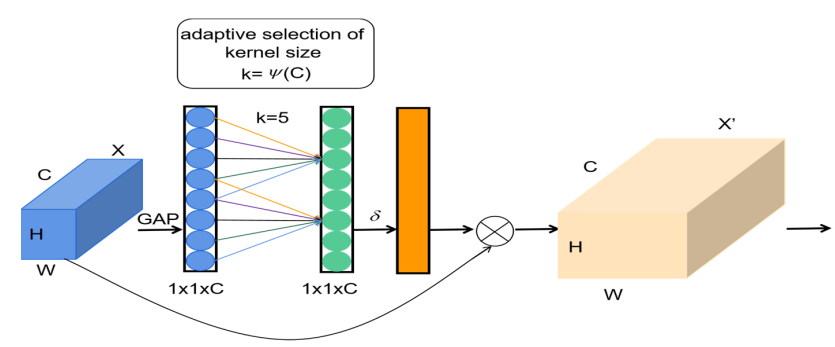
\includegraphics[width=0.9\textwidth]{appendices/images/FigureA9.png}
    \caption{ECA mechanism module \protect\parencite{hao2024squeezenet}.}
    \label{fig:ECA}
\end{figure}

Overall the model architecture is built upon a pretrained ResNet50, which serves as the backbone for feature extraction. The default fully connected layer is removed and replaced with a custom classification head that integrates an Efficient Channel Attention (ECA) mechanism. This mechanism enables the model to dynamically focus on the most informative regions of the input image, thereby enriching the feature representation with global context. To reduce overfitting, a dropout layer with a rate of 0.3 is applied before the final classification layer, which transforms the 2048-dimensional feature vector into predictions across the eight target classes.





\subsubsection{Classification:}  
After applying attention, the model includes a classification head that consists of:
\begin{itemize}
    \item \textbf{Dropout layer:} Helps prevent overfitting by randomly disabling some neurons during training.
    \item \textbf{Flatten layer:} Converts the 2D feature maps into a 1D vector.
    \item \textbf{Fully connected (FC) layer:} A linear layer that maps the extracted and attended features to class logits.
\end{itemize}

For training, the loss function used is the Cross-Entropy Loss with label smoothing, which mitigates model overconfidence by preventing overly peaked predictions \parencite{szegedy2016rethinking}. The smoothed loss function is defined in equation~\ref{eq:label_smoothing} as a combination of the standard cross-entropy loss (Equation~\ref{eq:cross_entropy}) and a uniform distribution over all $K$ classes::

\begin{equation}
L_{\text{smooth}} = (1 - \varepsilon) \cdot L_{\text{CE}} + \frac{\varepsilon}{K}
\label{eq:label_smoothing}
\end{equation}

\begin{equation}
L_{\text{CE}} = \sum_{i=1}^{K} y_i \log(p_i)
\label{eq:cross_entropy}
\end{equation}

Where:
\begin{itemize}
  \item $K$: Number of classes
  \item $y_i$: 1 if the true class is $i$, otherwise 0
  \item $p_i$: Predicted probability for class $i$
  \item $\varepsilon$: Smoothing factor (0.1)
\end{itemize}


The optimization process relies on Stochastic Gradient Descent (SGD), which proved to be more effective than the Adam optimizer, as demonstrated by the results presented in the following chapter in this section~\ref{sec:TestCnnM2}. To make the training faster and more stable, we also used two techniques: momentum and weight decay.

Momentum helps the model learn more smoothly and quickly. Instead of using only the current gradient (which shows the direction to update the model), momentum also takes into account the previous updates. This helps avoid getting stuck or bouncing too much when learning.

The update steps for SGD with momentum, as explained by \parencite{loshchilov2016sgdr}, are shown in Equation~\ref{eq:sgd_momentum}:

\begin{align}
v_{t+1} &= \mu v_t + \eta \nabla w_t \\
w_{t+1} &= w_t - v_{t+1}
\label{eq:sgd_momentum}
\end{align}

Where:  
\begin{itemize}
  \item \( v_t \): the velocity, which keeps track of the previous updates (momentum)
  \item \( \mu \): momentum factor (we used 0.9)
  \item \( \eta \): learning rate (we started with 0.001)
  \item \( \nabla w_t \): the gradient (how much the weights should change)
\end{itemize}


To mitigate overfitting, weight decay (L2 regularization) is applied with a coefficient set to $10^{-5}$ to penalize large weights and promote simpler, more generalizable models.

Instead of maintaining a constant learning rate throughout training, a cosine annealing schedule is employed to adjust it dynamically. This schedule starts with larger learning rates to allow broader exploration of the loss landscape and gradually reduces them to smaller steps as training progresses, enabling precise fine-tuning near the optimum. The cosine shape of the decay curve ensures a smooth transition between exploration and exploitation phases, facilitating stable and efficient convergence.

The learning rate $\eta_t$ at epoch $t$ is given by equation~\ref{eq:cosine_lr} \parencite{loshchilov2016sgdr}.

\begin{equation}
\eta_t = \eta_{\min} + \frac{1}{2}(\eta_{\max} - \eta_{\min}) \left(1 + \cos\left(\frac{t}{T} \pi\right)\right)
\label{eq:cosine_lr}
\end{equation}



Where:  
\begin{itemize}
  \item $\eta_{\max}$: initial learning rate (0.001)
  \item $\eta_{\min}$: minimum learning rate (typically $10^{-5}$)
  \item $T$: total number of epochs ($T = 25$)
\end{itemize}

The model was trained for up to 25 epochs with a batch size of 16, using early stopping with a patience of 3 to prevent overfitting and reduce unnecessary training time. The final classification layer uses the Softmax activation function to output a probability distribution over the nine disease classes.

Figure~\ref{fig:Model3TrainingPerformance} below summarizes the learning behavior of the model:
\begin{itemize}
    \item \textbf{Loss Curves:} A consistent decrease in both training and validation losses over epochs, indicating proper fitting.
    \item \textbf{Accuracy Curves:} A steady increase reaching high accuracy on both training and validation sets, without significant divergence, suggesting that the model generalizes well without overfitting.
\end{itemize}

\begin{figure}[H] % 'H' needs \usepackage{float}
    \centering
    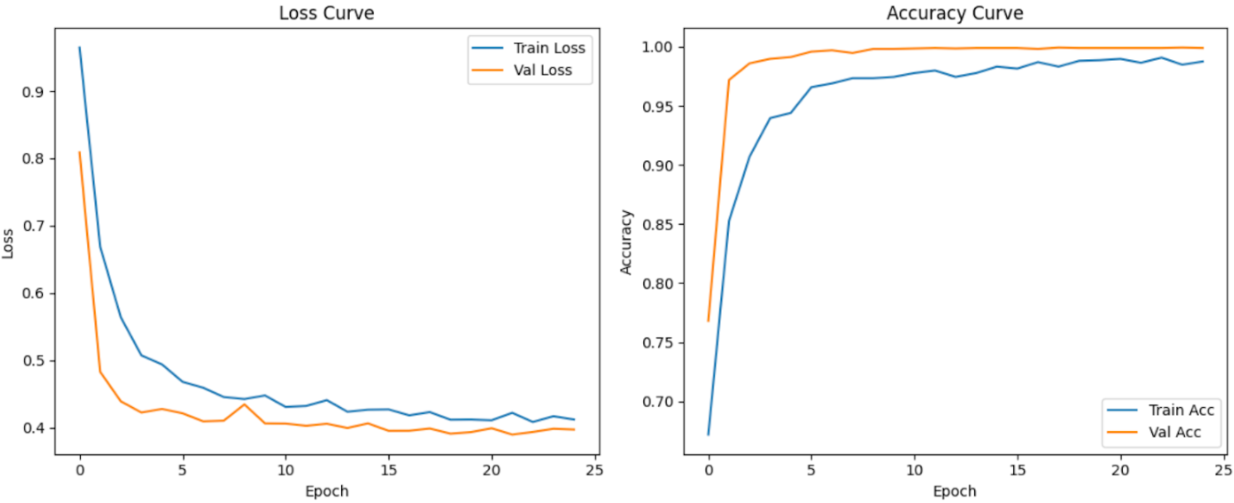
\includegraphics[width=0.9\textwidth]{chapters/chapter5/images/Figure03.png}
    \caption{Model 3 Training Performance: Loss and Accuracy Curves.}   ²²
    \label{fig:Model3TrainingPerformance}
\end{figure}

Once all components of the multi-class classification model M2 have been detailed, we present the following algorithm to illustrate the complete workflow: 



\begin{algorithm}[H]
\caption{Multi-class Classification Model (M2)}
\textbf{Input:} Dataset $\mathcal{D} = \{(x_i, y_i)\}_{i=1}^{N}$, where $N$ is the total number of image samples, $x_i$ denotes the $i$-th image of a wheat plant, and $y_i$ is the corresponding multi-class label. Each label $y_i \in \{1, \dots, K\}$ represents one of the $K$ distinct disease categories, including multiples classes for different types of wheat diseases\;
\textbf{Output:} Trained deep learning model $\mathcal{M}$\;

\vspace{2mm}
\textbf{Step 1: Data Preprocessing and Augmentation}\;
Split $\mathcal{D}$ into training (70\%), validation (15\%), and test (15\%) sets using stratified sampling\;

\textbf{Training set preprocessing pipeline:}\;
\Indp
Resize image to $512 \times 512$\; 
Random crop to $448 \times 448$\;
Apply geometric transformations:\;
\Indp
Horizontal and vertical flipping\;
Random rotation\;
Random shift, scale, and rotate\;
\Indm
Apply color augmentations:\;
\Indp
Random brightness and contrast adjustment\;
Hue, saturation, and value shifts\;
\Indm
Apply noise and blur:\;
\Indp
Gaussian blur\;
\Indm
Normalize image using ImageNet mean and std\;
Convert to tensor\;
\Indm

\textbf{Validation and test set preprocessing:}\;
\Indp
Resize to $512 \times 512$\;
Normalize with ImageNet statistics\;
Convert to tensor\;
\Indm

\vspace{2mm}
\textbf{Step 2: Feature Extraction and Classification}\;
Load pretrained ResNet-50 and remove its classification head\;
\ForEach{image $x_i$}{
    Extract feature map $F \in \mathbb{R}^{H \times W \times C}$ from ResNet-50, where $H$ and $W$ represent the height and width of the feature map, respectively, and $C$ denotes the number of channels.
    Apply Efficient Channel Attention (ECA) to refine $F$, yielding $F'$\;
    Flatten $F'$, apply Dropout, and use a fully connected layer to predict k-class output\;
}

\vspace{2mm}
\textbf{Step 3: Loss and Optimization}\;
Use Label Smoothing Cross-Entropy loss\;

Initialize Stochastic Gradient Descent (SGD) optimizer with learning rate scheduling (Cosine Annealing)\;

\vspace{2mm}
\textbf{Step 4: Training Strategy}\;
Train the model for a predefined number of epochs\;
Apply early stopping based on validation loss and accuracy\;

\vspace{2mm}
\textbf{Return:} Final trained model $\mathcal{M}$\;
\end{algorithm}



\section{Extending the proposed solution with insect pest detection and AI assistant for Proactive Intervention}
To improve the practicality and scope of the wheat disease classification system, two additional modules were added: insect pest detection and an AI assistant. The pest detection module identifies insects that may cause or spread diseases, allowing for early intervention. The AI assistant helps users understand the classification outcomes and get answers to their questions, making the system more accessible and actionable for farmers.

\subsection{Wheat insect pest dataset construction}

To train and evaluate the insect pest detection module, a dedicated dataset focusing specifically on pests that commonly affect wheat crops was constructed. The dataset includes high-quality images of various wheat-specific insect pests. Images were collected from publicly available agricultural databases, scientific publications, and a verified open-source dataset.
A preliminary review was conducted to identify existing datasets that could be repurposed for wheat pest detection. The table below (Table~\ref{tab:agricultural-pest-datasets}) summarizes the main publicly available insect pest datasets relevant to agriculture:

\begin{table}[htbp]
    \caption{Review of Existing Datasets for Agricultural Pest Detection}
    \centering
    \begin{tabular}{|p{4cm}|p{4cm}|p{5cm}|}
    \hline
    \textbf{Dataset Name} & \textbf{Crop Focus} & \textbf{Insect Species} \\
    \hline
    IP102 & Multiple crops & 102 classes \\
    \hline
    AgriPest & Rice, maize & 14 insect classes \\
    \hline
    D0C-Pest & Cotton & Cotton-specific insect pests \\
    \hline
    Deep Weeds & Weeds in pastures & Weed species only \\
    \hline
    \end{tabular}
    \label{tab:agricultural-pest-datasets}
\end{table}


These available datasets were generally designed for a wide range of agricultural pests. However, since our focus is on wheat-specific pests, only the subsets relevant to wheat were selected and extracted. This selective approach allowed us to construct a custom dataset tailored to our objectives, as shown in Table~\ref{tab:target-pest-classes}. The constructed dataset satisfies the following criteria:

\begin{itemize}
    \item \textbf{Wheat-specific relevance:} All included pest images correspond to insect species known to affect wheat crops, ensuring high domain specificity.
    \item \textbf{Diversity of conditions:} The dataset includes images captured under various lighting, background, and environmental conditions to enhance model robustness.
    \item \textbf{Quality and clarity:} Only high-resolution images with clear visibility of the target pests were selected to support accurate detection and annotation.
    \item \textbf{Multi-class:} Covers multiple pest species in both adult and larval stages.
    \item \textbf{Accurate annotations:} Each image was manually annotated with oriented bounding boxes and class labels using standard tools to ensure precise localization.
\end{itemize}


\begin{table}[htbp]
    \caption{Target Pest Classes and Biological Relevance}
    \centering
    \begin{tabular}{|p{4cm}|p{6cm}|}
    \hline
    \textbf{Pest classes}  & \textbf{Number of images} \\
    \hline
    Armyworm Moth  & 314 \\
    \hline
    Armyworm Larvae & 223 \\
    \hline
    Aphid &  307 \\
    \hline
    Grasshopper  & 216 \\
    \hline
    Mite &  278 \\
    \hline
    Beetle  & 188 \\
    \hline
    Sawfly & 165 \\
    \hline
    \textbf{Total} & \textbf{1691} \\
    \hline
    \end{tabular}
    \label{tab:target-pest-classes}
\end{table}

To produce accurate annotations for supervised object detection, the CVAT (Computer Vision Annotation Tool) was deployed locally using Docker. This setup enabled collaborative annotation and allowed exporting in various formats. The following figure (Figure~\ref{fig:CVATAnnotation}) showcases annotated images for each insect pest class in the dataset.


\begin{figure}[H] % 'H' needs \usepackage{float}
    \centering
    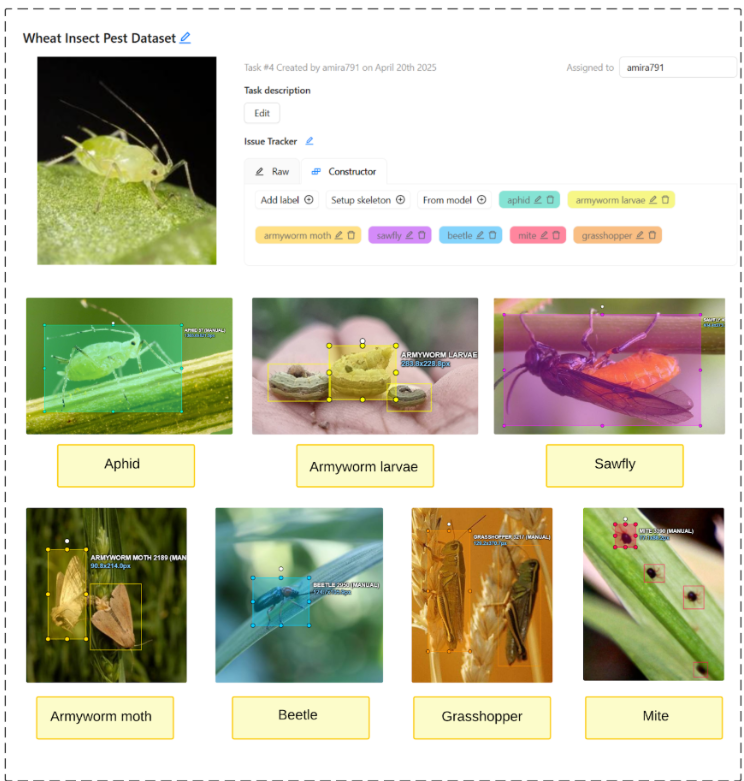
\includegraphics[width=0.9\textwidth]{chapters/chapter4/images/Figure08.png}
    \caption{Wheat insect pest annotation task in CVAT.}
    \label{fig:CVATAnnotation}
\end{figure}


\subsection{YOLOv8m-OBB for Insect Pest Detection}

To detect insect pests in wheat field images with high accuracy, we adopted the YOLOv8m-OBB model provided by Ultralytics (Refer to Appendix~\ref{app:annexA} for details). This architecture supports oriented bounding boxes (OBBs), making it highly suitable for localizing small, variably-angled pests in real-world scenes.

Unlike traditional horizontal bounding boxes (HBBs) that align strictly with the image axes, OBBs provide tighter and more accurate localization for irregularly shaped or rotated pests (see Figure~\ref{fig:obb_vs_hbb}). During the annotation phase, we followed a two-step approach to compare the performance of different bounding strategies:

\begin{itemize}
\item First, the dataset was annotated using horizontal bounding boxes (HBBs), and we trained a standard YOLOv8 model on this version.
\item Next, we re-annotated the same dataset using oriented bounding boxes (OBBs), and trained the YOLOv8m-OBB model adapted for quadrilateral outputs.
\end{itemize}

The comparison revealed that the YOLOv8m-OBB model significantly outperformed the standard YOLOv8 in both precision and robustness. The OBB annotations enabled better localization of pests, particularly in cases of rotation, occlusion, and cluttered backgrounds. (See the results in the Section~\ref{sec:Pesttest}).

\paragraph{Model Architecture:}

The YOLOv8m-OBB follows the general structure of YOLOv8 with key adaptations for OBB prediction:

\begin{itemize}
\item \textbf{Backbone:} A CSPDarknet-inspired backbone extracts meaningful visual features using convolutional layers, residual connections, and cross-stage partial connections (CSP).
\item \textbf{Neck:} A Path Aggregation Network (PANet) fuses features across scales in both bottom-up and top-down paths. This enables the combination of:
\begin{itemize}
    \item \textbf{Low-level features}: Fine texture details useful for detecting small pests.
    \item \textbf{High-level features}: Semantic abstraction for accurate classification.
\end{itemize}

\item \textbf{Detection Head:} The main distinction lies here. 
\begin{itemize}
    \item In standard YOLOv8, the head outputs class labels, objectness scores, and four coordinates \((x, y, \text{width}, \text{height})\).
    \item In YOLOv8m-OBB, the head is modified to output eight coordinates \((x_1, y_1, x_2, y_2, x_3, y_3, x_4, y_4)\), representing a quadrilateral that can rotate and skew to match pest orientation. This is critical in field conditions where:
    \begin{itemize}
        \item Pests may appear at arbitrary angles.
        \item Partial occlusion and complex backgrounds are common (e.g., wheat leaves).
        \item Regular boxes can include excessive background, reducing precision.
    \end{itemize}
\end{itemize}
\end{itemize}

\begin{figure}[H]
\centering
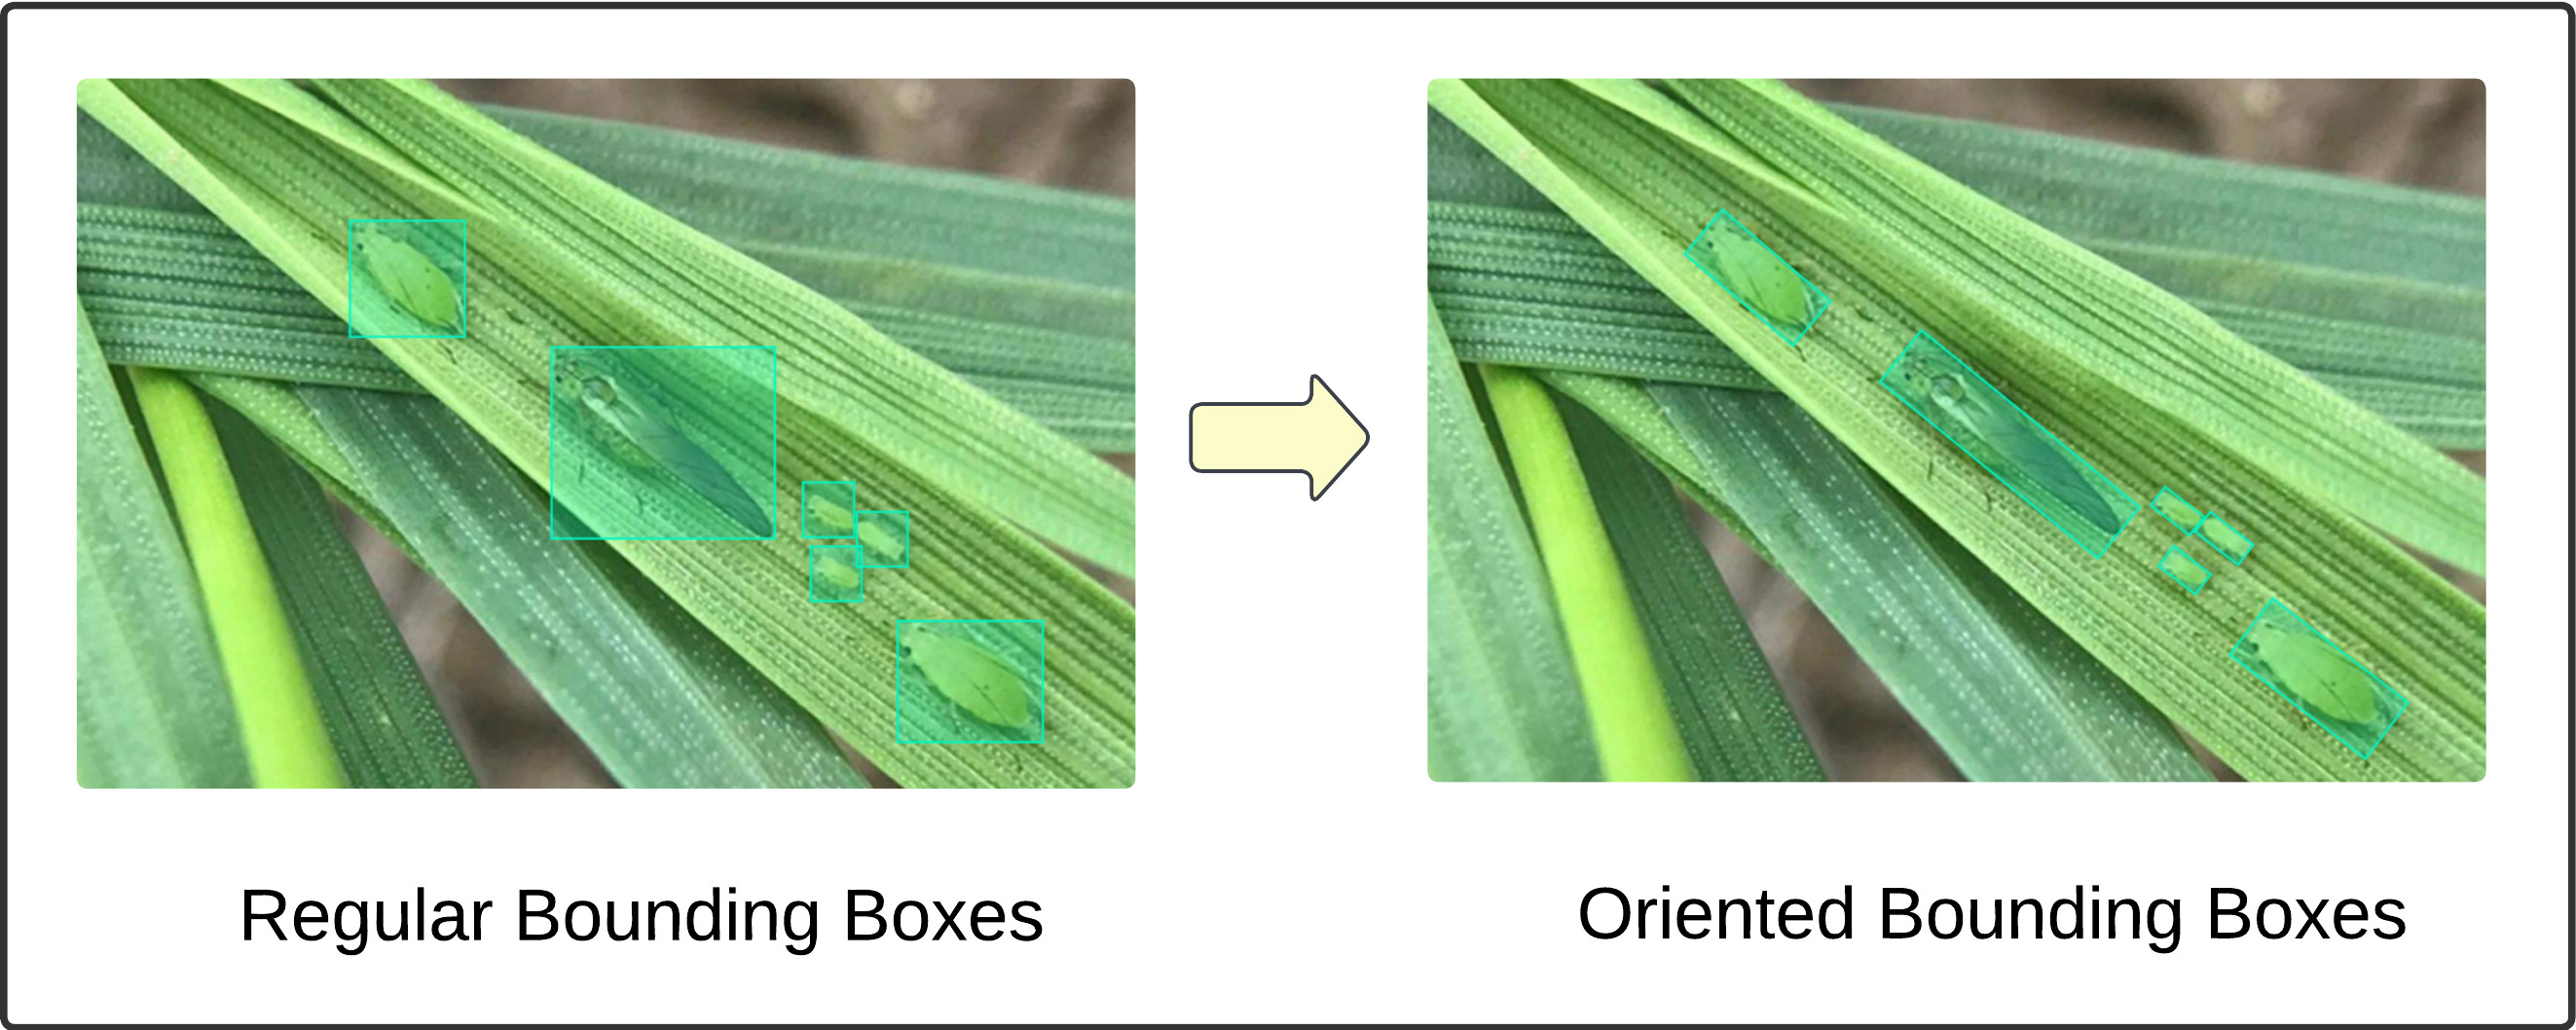
\includegraphics[width=0.9\textwidth]{chapters/chapter4/images/Figure13.jpeg}
\caption{Comparison between regular bounding boxes and oriented bounding boxes.}
\label{fig:obb_vs_hbb}
\end{figure}



\subsubsection{Data preparation and annotation}

The original dataset consisted of 1,691 high-resolution field images, containing a total of 3,796 annotated pest instances. The annotation was performed using the CVAT tool (Computer Vision Annotation Tool), exported in the Ultralytics YOLO Oriented Bounding Boxes 1.0 format, which includes the object class and the eight coordinates of the OBB.

To ensure proper training structure, an 80/20 train-test split was conducted using a custom Python script. The dataset was organized to fit the YOLO training format. A summary of the split is shown in Table~\ref{tab:split}.

\begin{table}[h]
\centering
\caption{Dataset split summary}
\begin{tabular}{|c|c|c|}
\hline
\textbf{Subset} & \textbf{Number of Images} & \textbf{Number of Annotations} \\
\hline
Training & 1346 & 3315 \\
Testing & 345 & 481 \\
\hline
\textbf{Total} & \textbf{1691} & \textbf{3796} \\
\hline
\end{tabular}
\label{tab:split}
\end{table}

A preprocessing step was performed to clean and verify the annotation files:
\begin{itemize}
    \item Malformed entries were removed.
    \item Coordinates were clipped to stay within the normalized \([0,1]\) range.
    \item Label format was standardized for consistency.
\end{itemize}

\subsubsection{Data augmentation techniques}

To increase model generalization and robustness to environmental variability (e.g., lighting, pest pose, occlusion), several augmentations were applied during training, as shown in Table~\ref{tab:augmentations}.


\begin{table}[H]
    \caption{Data Augmentation Techniques and Their Roles.}
    \centering
    \begin{tabular}{|p{5cm}|p{8cm}|}
    \hline
    \textbf{Augmentation Technique (Value)} & \textbf{Role} \\
    \hline
    Image Rotation (45°) & Simulates various object orientations in real scenes. \\
    \hline
    Horizontal Flip (0.5) & Mirrors images horizontally to reduce bias in object direction. \\
    \hline
    Vertical Flip (0.5) & Flips images vertically to enhance variability and robustness. \\
    \hline
    MixUp (0.2) & Blends two images and their labels to regularize the model. \\
    \hline
    Copy-Paste (0.2) & Copies objects from one image to another to simulate occlusion and increase density. \\
    \hline
    Hue Variation (0.015) & Adjusts image color hue to improve robustness under different lighting conditions. \\
    \hline
    Saturation Variation (0.7) & Changes color intensity to handle lighting and environmental variation. \\
    \hline
    Brightness Variation (0.4) & Modifies brightness to simulate varying exposure and shadows. \\
    \hline
    \end{tabular}
    \label{tab:augmentations}
\end{table}


\subsubsection{Model training configuration}

The YOLOv8m-OBB model was trained over 300 epochs using optimized parameters that balance performance and resource consumption. Table~\ref{tab:train-config} summarizes the main training settings.
\begin{table}[H]
    \caption{YOLOv8m-OBB Training Configuration and Parameter Roles}
    \centering
    \begin{tabular}{|p{6cm}|p{9cm}|}
    \hline
    \textbf{Parameter (Value)} & \textbf{Role} \\
    \hline
    Model (YOLOv8m-OBB) & Pre-trained model variant supporting oriented bounding boxes for better detection of rotated objects. \\
    \hline
    Epochs (300) & Maximum number of training cycles; training stopped early at 201 epochs due to early stopping. \\
    \hline
    Batch Size (16) & Number of images processed together in one training iteration; affects speed and stability. \\
    \hline
    Image Size (640 × 640) & Input image resolution used during training; balances detail and computation. \\
    \hline
    Optimizer (AdamW) & Optimization algorithm combining Adam with weight decay to improve generalization. \\
    \hline
    Initial Learning Rate (0.001) & Starting step size for updating model weights. \\
    \hline
    Learning Rate Factor (0.01) & Minimum learning rate as a fraction of the initial rate (used in cosine annealing). \\
    \hline
    Weight Decay (0.0005) & Regularization term to prevent overfitting by penalizing large weights. \\
    \hline
    Patience (50) & Number of epochs with no improvement before triggering early stopping. \\
    \hline
    Number of Workers (4) & Number of parallel processes used for data loading. \\
    \hline
    Objectness Weight (2.0) & Balances the importance of objectness confidence during training. \\
    \hline
    \end{tabular}
    \label{tab:train-config}
\end{table}
  


\subsection{AI Assistant Integration for Interactive Agricultural Intelligence}

To enhance the usability and impact of the proposed system, an AI assistant module was integrated into the web platform. This conversational interface enables farmers to interact naturally with the platform by submitting either text queries or images with brief descriptions. They can inquire about wheat diseases, pest identification, suitable treatments, or general agricultural practices. The assistant provides accurate, context-aware responses, helping even non-expert users make informed decisions with confidence.

The chatbot is powered by the Gemini API on the Google Cloud Platform (GCP), which uses a large language model (LLM) capable of understanding and generating detailed responses to agricultural queries. It supports two types of user input:
\begin{itemize}
\item \textbf{Text queries}: For describing symptoms or requesting advice.
\item \textbf{Image + text}: For more precise, context-rich diagnoses.
\end{itemize}

The system ensures secure and efficient communication between the user interface and Gemini’s inference endpoint via API calls, enabling real-time, intelligent interactions embedded directly within the agricultural support platform.

Figure~\ref{fig:ai_assistant_integration} illustrates the overall workflow of this integration, which empowers users with immediate access to practical and reliable insights.

\begin{figure}[H]
\centering
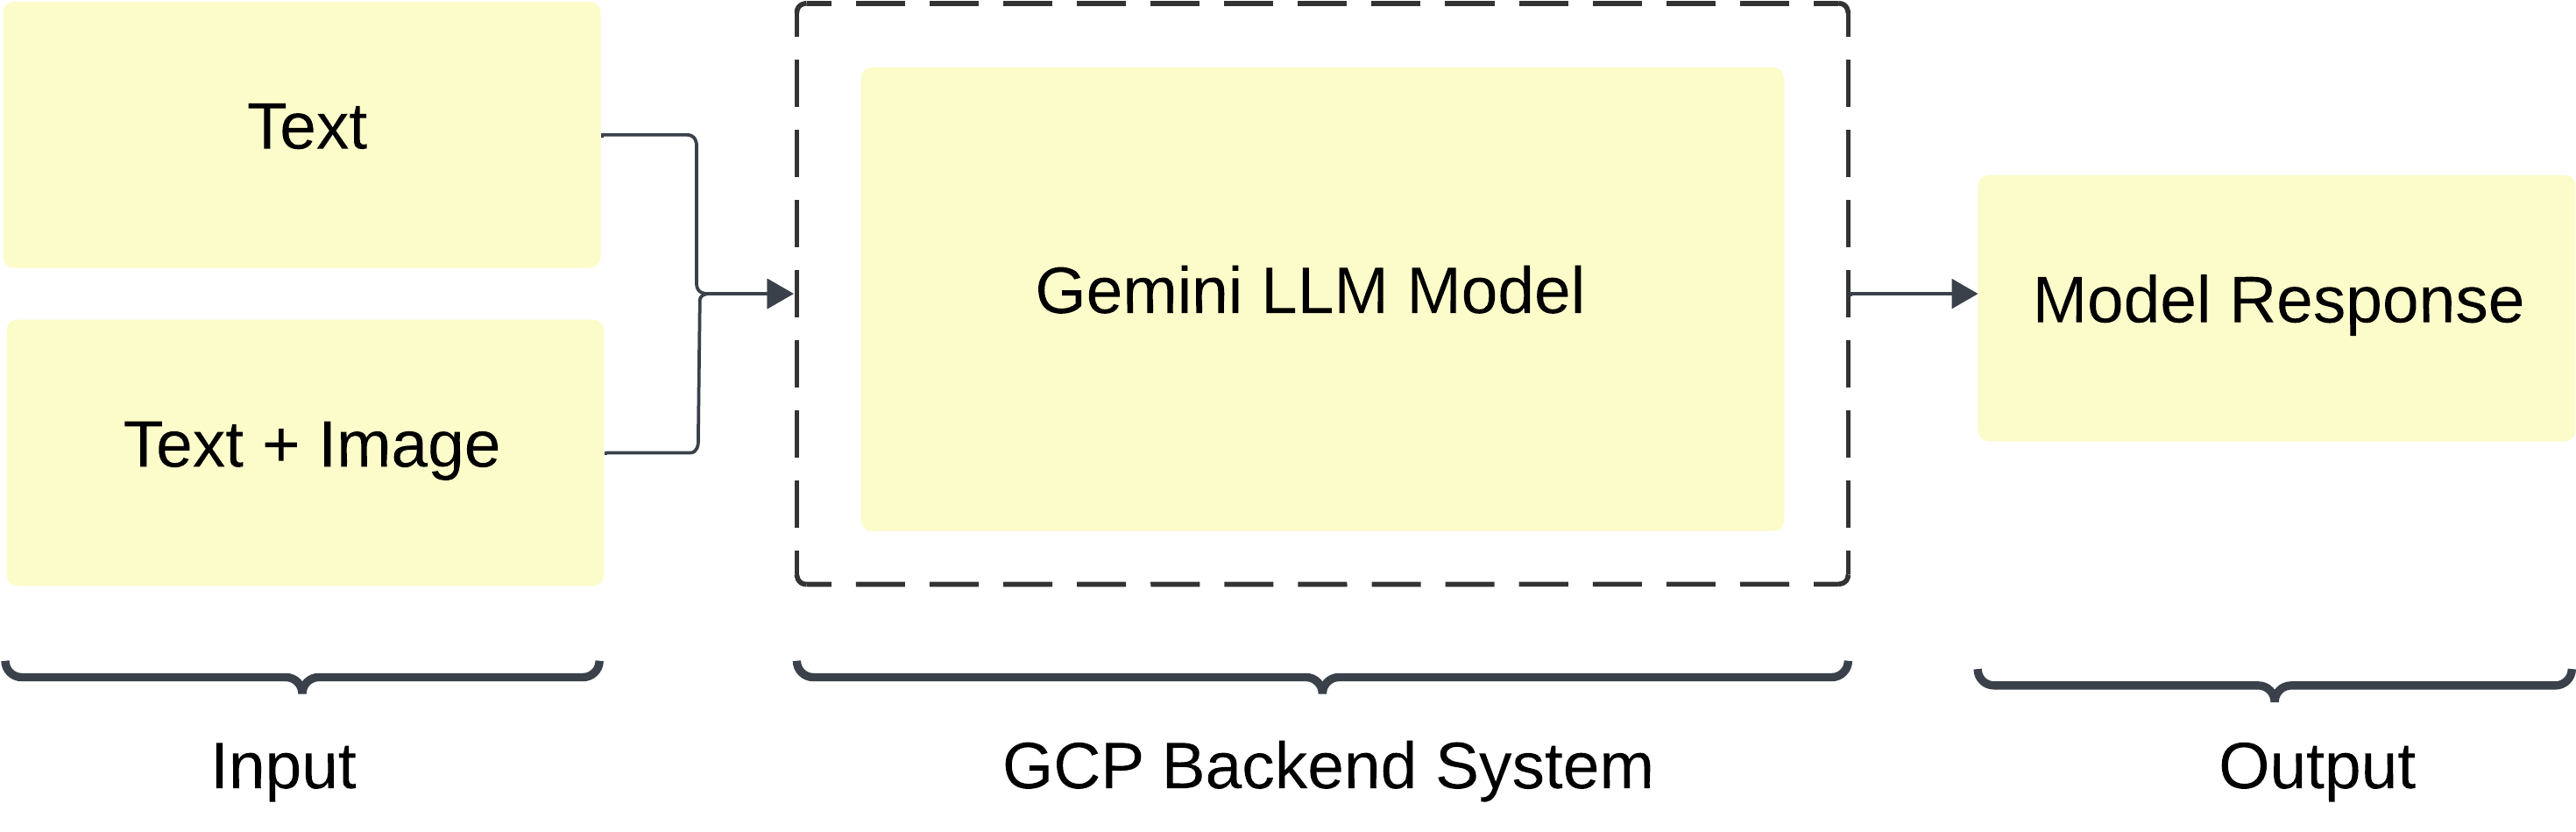
\includegraphics[width=0.9\textwidth]{chapters/chapter4/images/Figure14.png}
\caption{AI assistant integration workflow.}
\label{fig:ai_assistant_integration}
\end{figure}






















\section{Web platform design}
To ensure practical usability of the proposed system by end users such as farmers, agronomists, and researchers, a dedicated web platform was developed. This platform serves as the main interface for interacting with the AI-based crop health monitoring system, integrating both wheat disease classification and insect pest detection modules.
The platform was designed with a focus on simplicity, efficiency, and accessibility, allowing users to upload images, receive predictions, and visualize results with minimal effort. 



\subsection{Functional Specifications}
The functional requirements of our system are detailed in the table below using the MoSCoW method (Must M, Should S, Could C, Won’t W) to prioritize features based on their importance. This system is designed to assist farmers in classifying wheat diseases and identifying insect pests through an easy-to-use web application (see Table~\ref{tab:FunctionalSpecifications}).


\begin{table}[h!]
\centering
\caption{Functional specifications of the web platform}
\begin{tabular}{|c|p{12cm}|c|}
\hline
\textbf{ID} & \textbf{Requirement} & \textbf{Priority} \\
\hline
F1 & The system must allow the user to upload images and analyze them. & M \\
\hline
F2 & The system must allow the user to select a prediction task (Wheat disease classification, Insect pest detection). & M \\
\hline
F3 & The system must allow the user to visualize the result of the prediction, including annotated images and relevant classification or detection details. & M \\
\hline
F4 & The system must process the image using the appropriate trained model and display the prediction results. & M \\
\hline
F5 & The system must allow users to export(download) prediction result. & M \\
\hline
F6 & The system should provide a chatbot assistant to guide and support the user. & S \\
\hline
F7 & The system could provide a documentation section containing detailed descriptions of common wheat diseases and insect pests, including symptoms, impact, and treatment suggestions. & C \\
\hline
\end{tabular}
\label{tab:FunctionalSpecifications}
\end{table}



\subsection{Use case diagrams}
The use case diagram, based on UML standards, models the needs of users and provides an overview of the wheat monitoring system's functionalities. As shown in Figure~\ref{fig:usecase}, the primary users—such as farmers, agronomists, or researchers—interact with the system to monitor wheat health, identify pests, and receive predictions. They can select a prediction task, either insect pest detection or wheat disease classification, which requires uploading or dragging an image. Once the prediction is completed, users can visualize the results and optionally download a report. The system also includes a chatbot assistant for support and integrates with the Gemini API for backend processing.


\begin{figure}[H] % 'H' needs \usepackage{float}
    \centering
    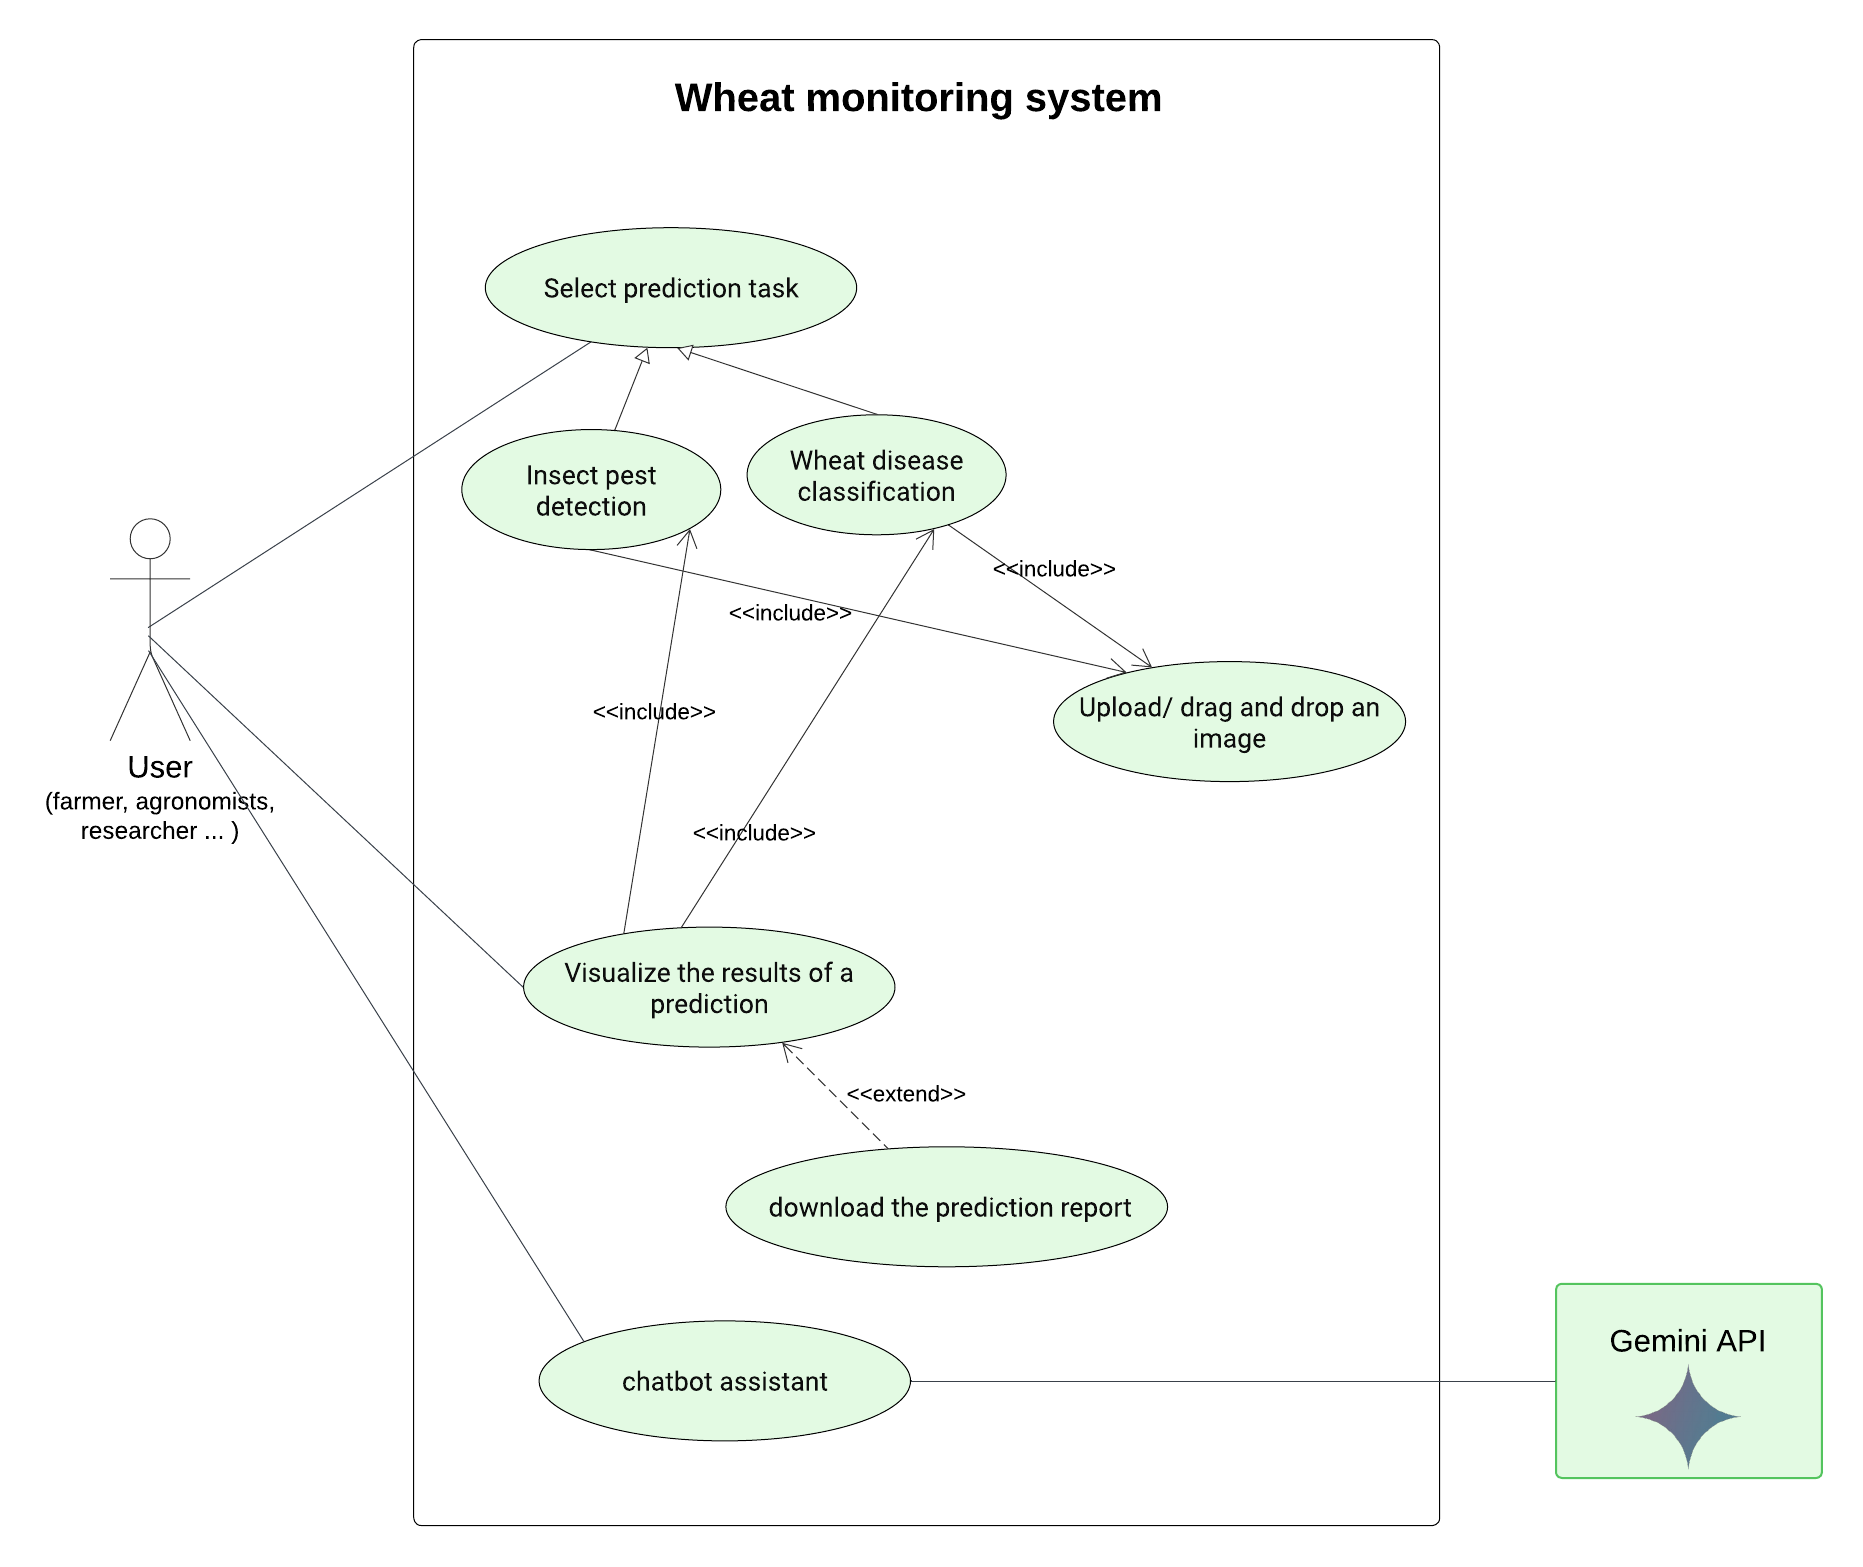
\includegraphics[width=0.9\textwidth]{chapters/chapter4/images/Figure10.png}
    \caption{The use case diagram of the system.}
    \label{fig:usecase}
\end{figure}

\subsection{Activity diagrams}

Activity diagrams provide a high-level view of the dynamic behavior of the system. They are particularly useful for illustrating the sequence of actions involved in performing specific tasks from a user perspective. In the context of our web platform, we developed two distinct activity diagrams (Figure~\ref{fig:ActivityDiagrams}), each corresponding to a core task of the system: wheat disease classification and wheat insect pest detection. These diagrams help visualize the user interaction flow, system responses, and processing steps for each use case. (see Figure~\ref{fig:usecase})


\begin{figure}[H] % 'H' needs \usepackage{float}
    \centering
    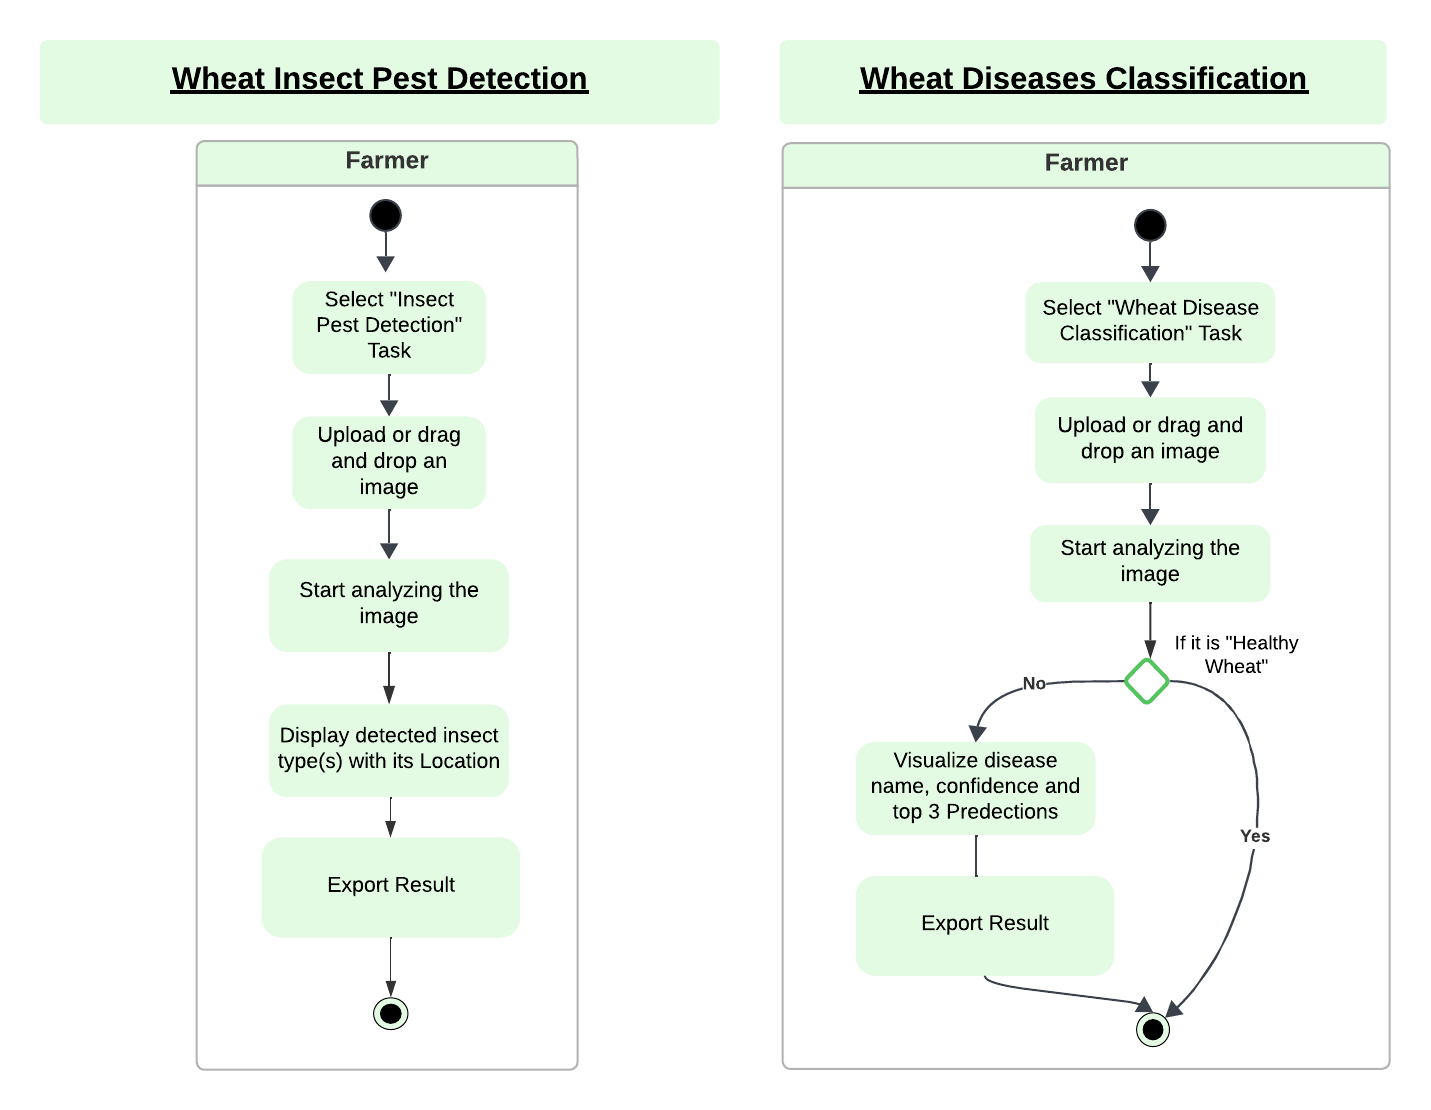
\includegraphics[width=\textwidth]{chapters/chapter4/images/Figure12.png}
    \caption{Activity diagrams for Wheat disease classification and insect pest detection}
    \label{fig:ActivityDiagrams}
\end{figure}


% \begin{figure}[H] % 'H' needs \usepackage{float}
%     \centering
%     
\includegraphics[width=0.9\textwidth]{chapters/chapter4/images/Figure11.png}
%     \caption{Activity Diagram for Wheat Disease Classification.}
%     \label{fig:ActivityDiagramWheat}
% \end{figure}



% \begin{figure}[H] % 'H' needs \usepackage{float}
%     \centering
%     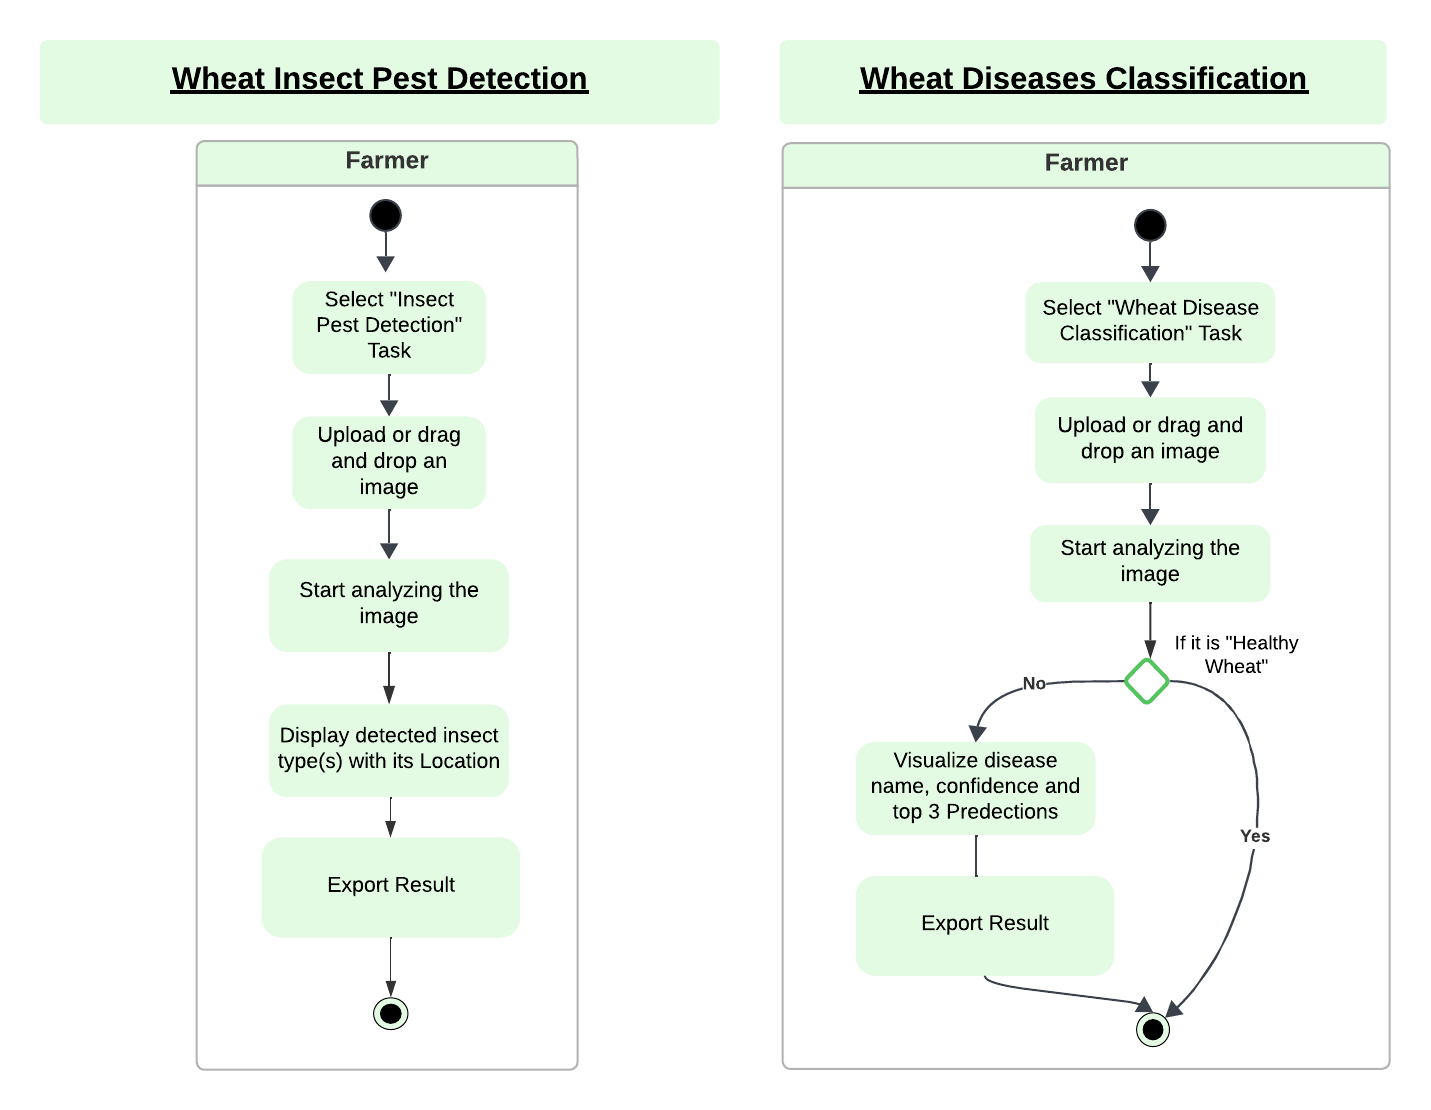
\includegraphics[width=0.9\textwidth]{chapters/chapter4/images/Figure12.png}
%     \caption{Activity Diagram for Wheat Insect Pest Detection.}
%     \label{fig:ActivityDiagramPest}
% \end{figure}



\section{Conclusion}
In this chapter, we explained the design of our solution for wheat disease classification and pest detection. We used advanced deep learning models and well-prepared datasets to build an effective system. We also included an AI assistant to improve the process.The architecture and web platform were designed to be both accurate and easy to use.

In the next chapter, we will show how we implemented this solution and tested it. The tests include performance evaluation and experiments to justify the design choices made for each model.

